\documentclass[12pt]{article}
\usepackage[utf8]{inputenc}
\usepackage{graphicx}
\usepackage{fixltx2e}
\graphicspath{{images/}}
\usepackage{float}
\usepackage[magyar]{babel}
\title{Rendszer- és irányításelmélet esti 2017-18 tavasz házi feladat}
\author{Benkő Gábor}
\date{\today}
\begin{document}
\maketitle
\newpage
\section{Empirikus szabályozótervezés}
\subsection{Szabályozó tervezés Ziegler-Nichols kísérleti identifikáción alapuló szabályozás módszerével}
\begin{figure}[h]
    \centering
	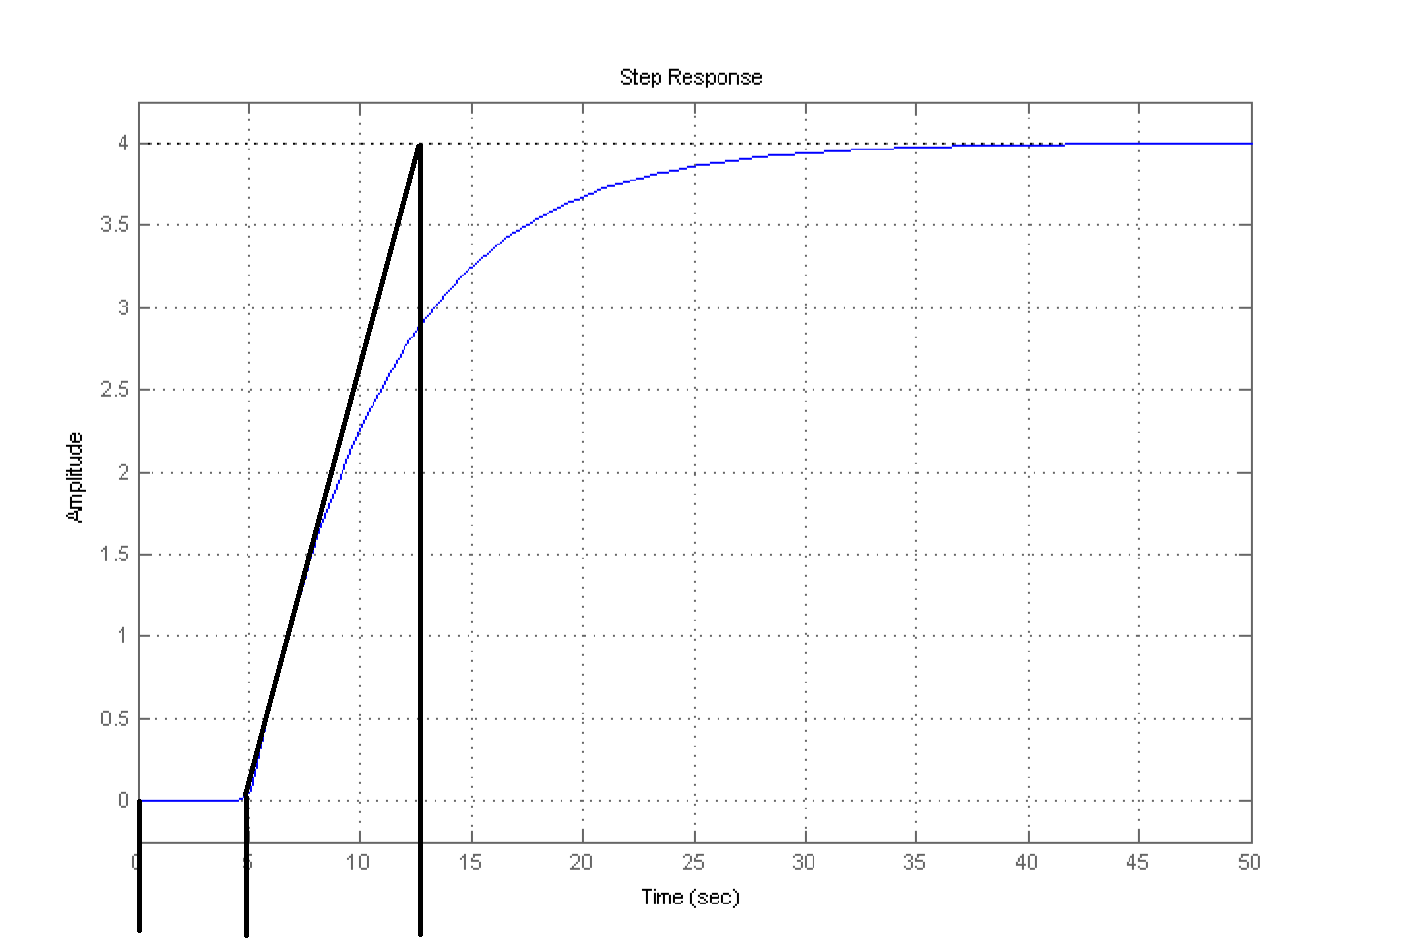
\includegraphics[scale=.4]{stepresponse}
	\caption{A szabályozandó rendszer ugrásválasza}
	\label{fig:stepresponse}
\end{figure}
Az ábrán látható megadott ugrásválasz alapján kerül tervezésre a PID szabályozó. Az ugrásválasz alapján az identifikáció alapján az alábbi értékek kerültek kinyerésre:
\begin{center}
\begin{tabular}{|c c c|}
\hline Név & Jelölés & Érték \\
\hline \hline
Holtidő & T\textsubscript{u} & 4\textsubscript{s} \\
\hline
Felfutási idő & T\textsubscript{r} & 12\textsubscript{s} \\
\hline
A szakasz erősítése & K\textsubscript{p} & 4 \\
\hline
\end{tabular}
\end{center}
Az eredményekből kiszámolásra került a $\rho=\frac{T_u}{T_r}=\frac{4}{13}=0.3333$ értéke, illetve a $T_I=2*T_U=8$ és a $T_D=T_U=4$. Az $A_p$ értéke kiszámolása a $A_p*K_p*\rho\leq1.2$ egyenlet átrendezésével \[A_P\leq\frac{1.2}{K_P*\rho}\leq0.9000\]
A PID szabályozó átviteli függvénye \[W\textsubscript{PID}=0.9000*(1+\frac{1}{8s}+4s)\]
ahol a MATLAB alapján keletkezett átviteli függvény \[W\textsubscript{PID}=\frac{3.6s^2+0.9s+0.1125}{s}\].
A Simulink-ban létrehozott rendszer ugrásválasza:
\begin{figure}[H]
\centering
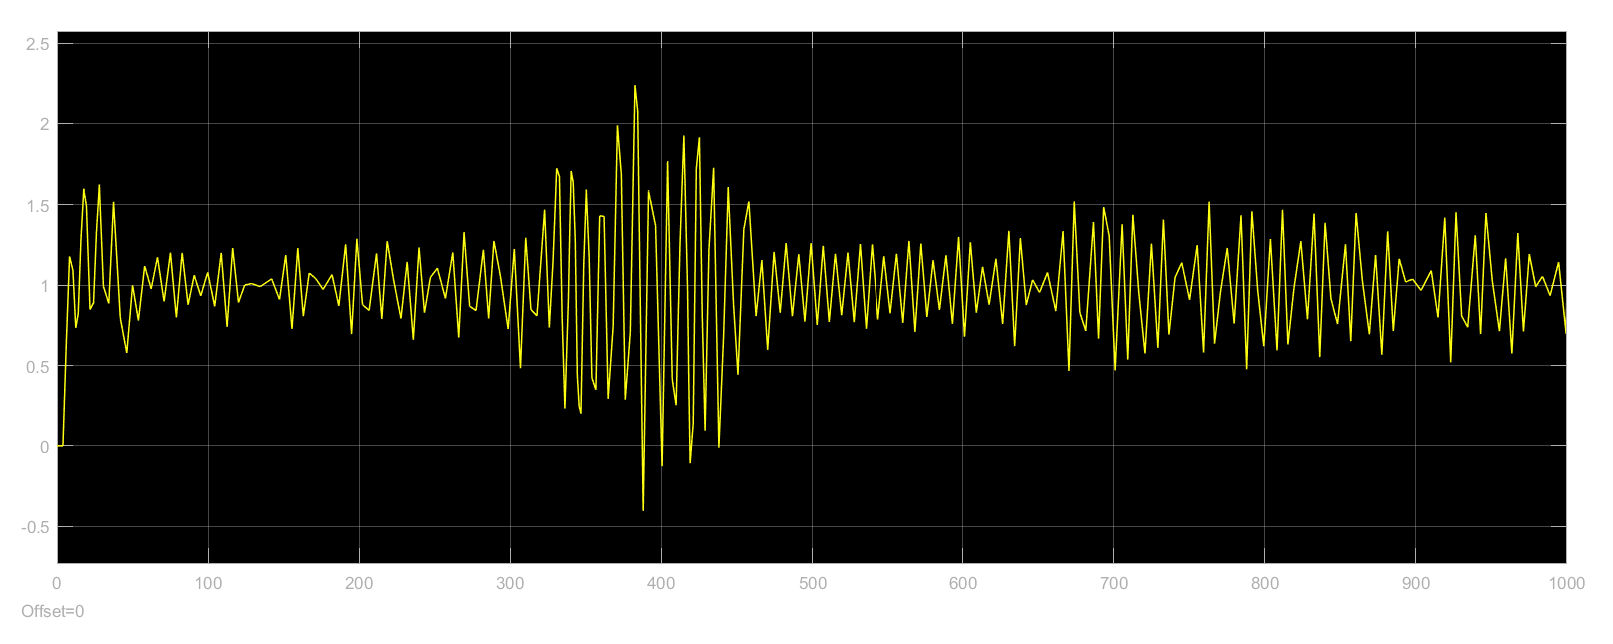
\includegraphics[scale=.50]{zgpidosc}
\caption{Az $A_P=0.9000$ rendszer ugrásválasza}
\end{figure}
Az ugrásválasz alapján látható a rendszer a stabilitás határán van. Ha rendszer stabilan szeretnénk tartani akkor $A_P<0.9000$ kell lennie. Így empirikus módszer segítségével csökkentjük az erősítési tényezőt, amíg megtaláljuk a közeli erősítési tényezőt.
A felezési módszertannal $A_P=0.1000$ esetén:
\begin{figure}[H]
\centering
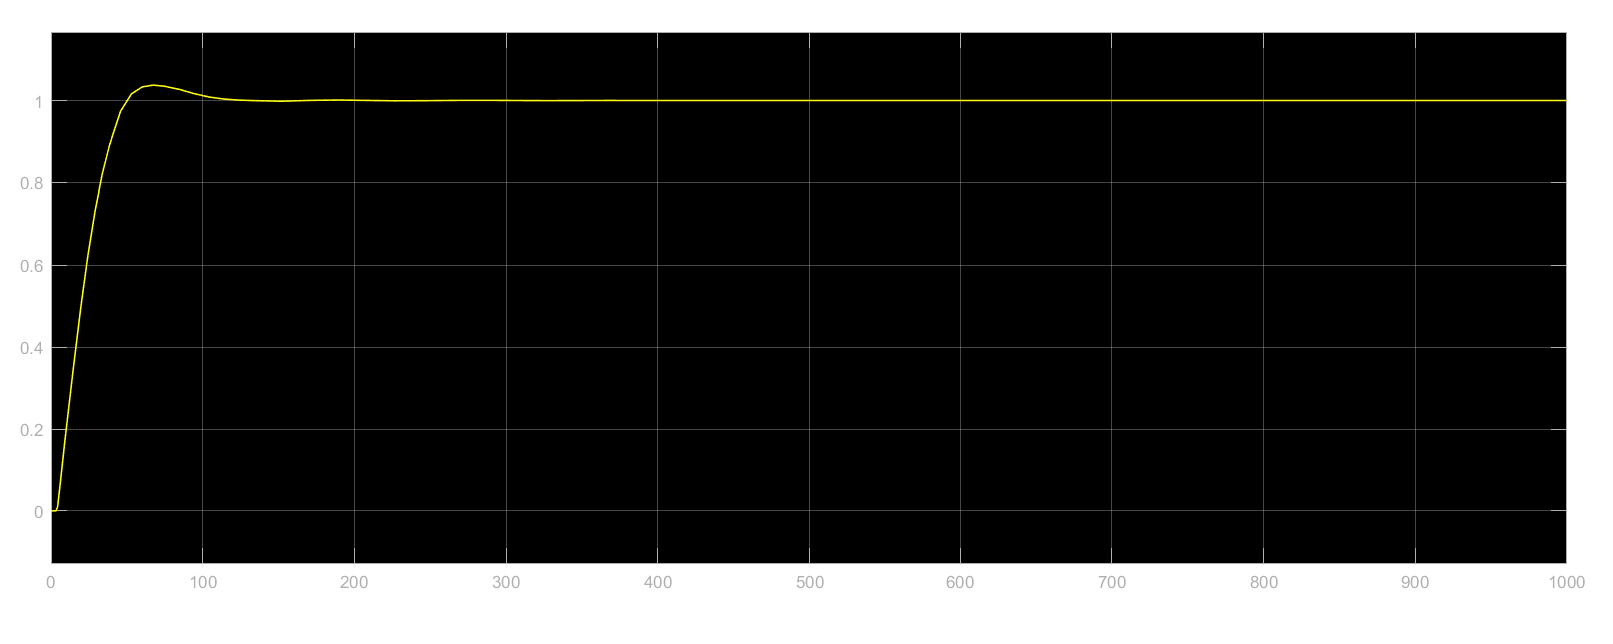
\includegraphics[scale=.50]{ap0100}
\caption{Az $A_P=0.1000$ rendszer ugrásválasza}
\end{figure}
a rendszerünk már stabil, illetve van egy kis túllövése, mely után beáll állandósult állapotba. A rendszer erősítését így tovább növelhetjük. A felezési módszer alapján, most az $A_P=0.4500$ erősítés esetén:
\begin{figure}[H]
\centering
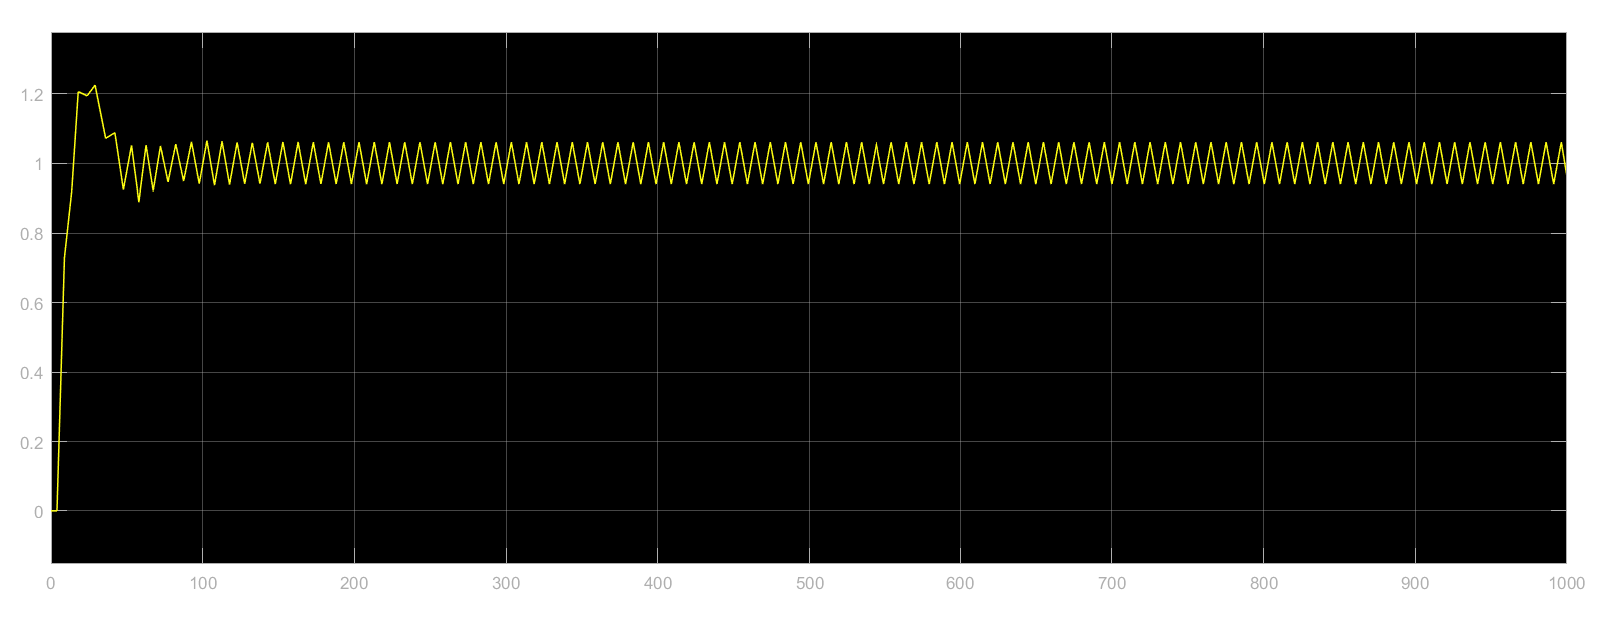
\includegraphics[scale=.50]{ap0450}
\caption{Az $A_P=0.4500$ rendszer ugrásválasza}
\end{figure}
A rendszer most a stabilitás határán van, így az erősítés tényezőt csökkentem $A_P=0.225$ értékre.
\begin{figure}[H]
\centering
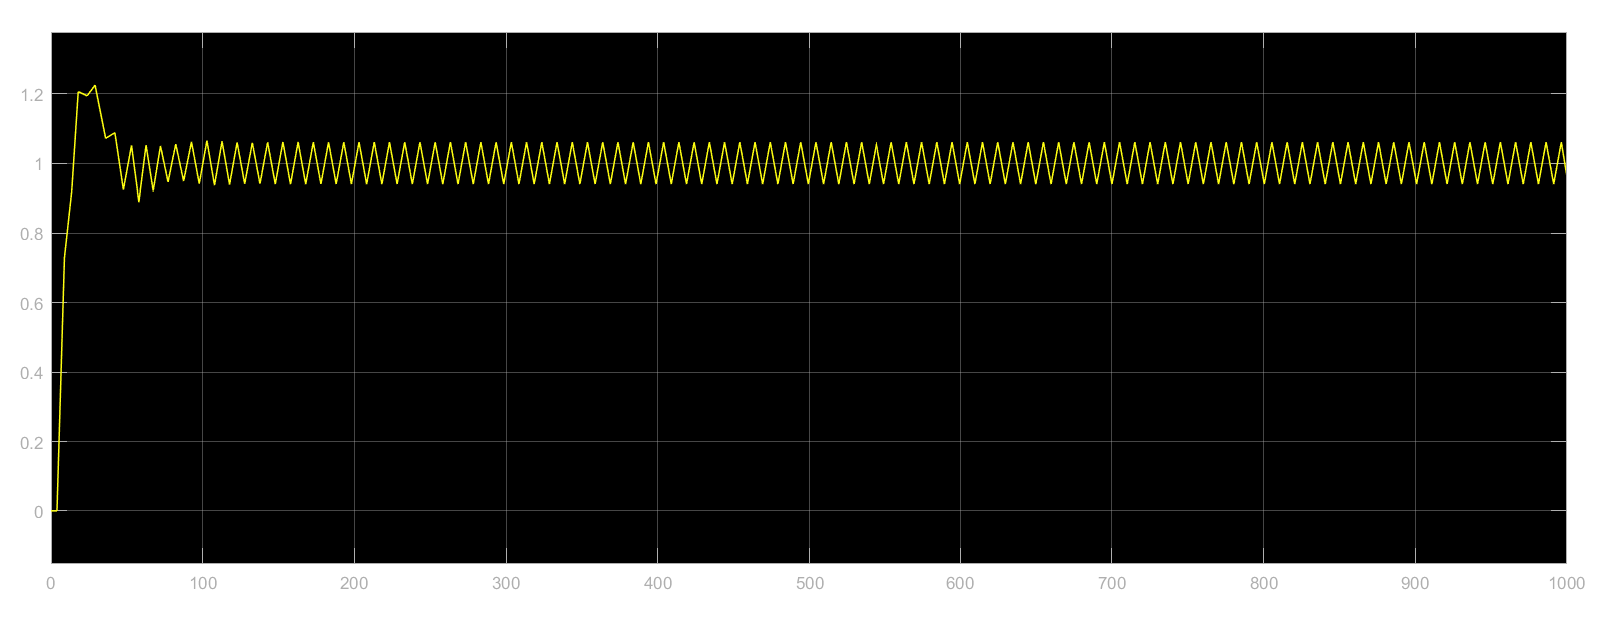
\includegraphics[scale=.50]{ap0450}
\caption{Az $A_P=0.2250$ rendszer ugrásválasza}
\end{figure}
A rendszer $A_P=0.2250$ estén stabil és van túllövése. Az $A_P$ értéke növelhető $A_P=0.337$.
\begin{figure}[H]
\centering
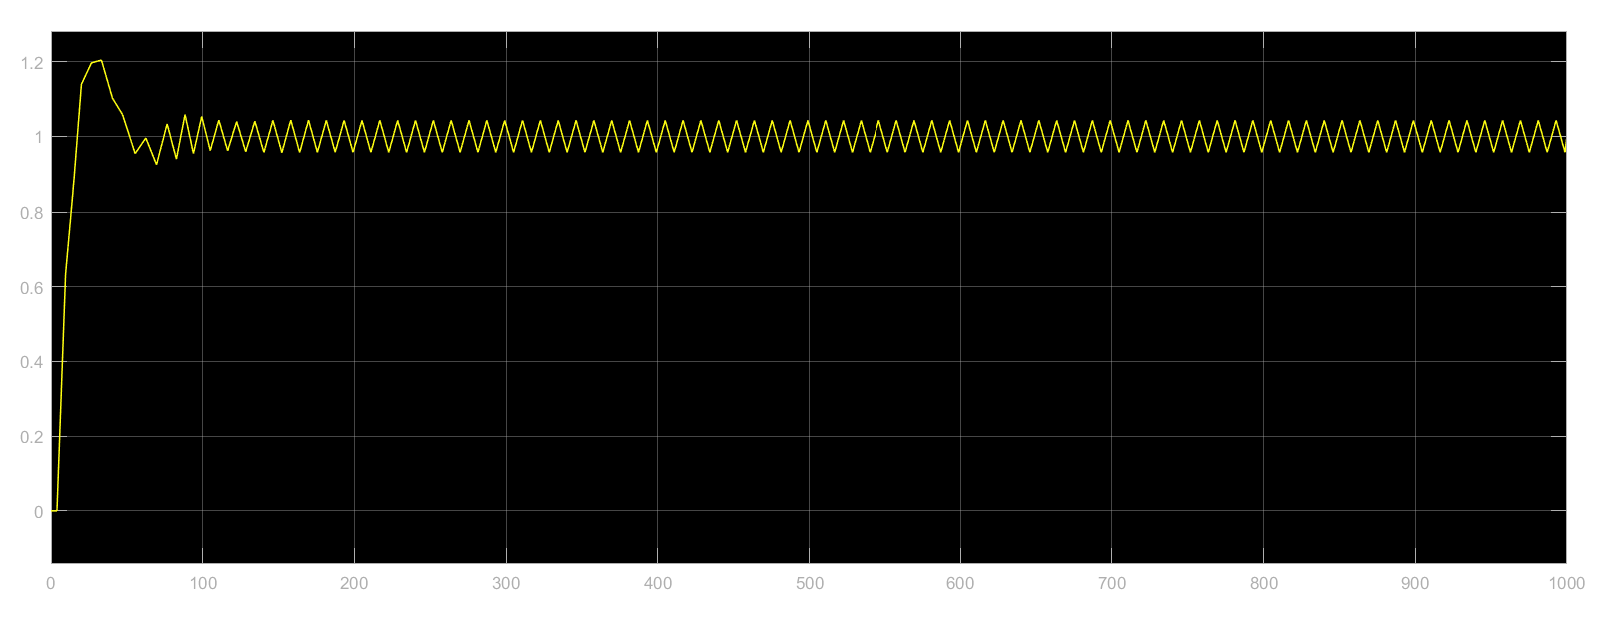
\includegraphics[scale=.50]{ap337}
\caption{Az $A_P=0.3370$ rendszer ugrásválasza}
\end{figure}
A rendszer a stabilitás határán van, így az $A_P=0.2810$ értékre csökkentve az ugrásválasz:
\begin{figure}[H]
\centering
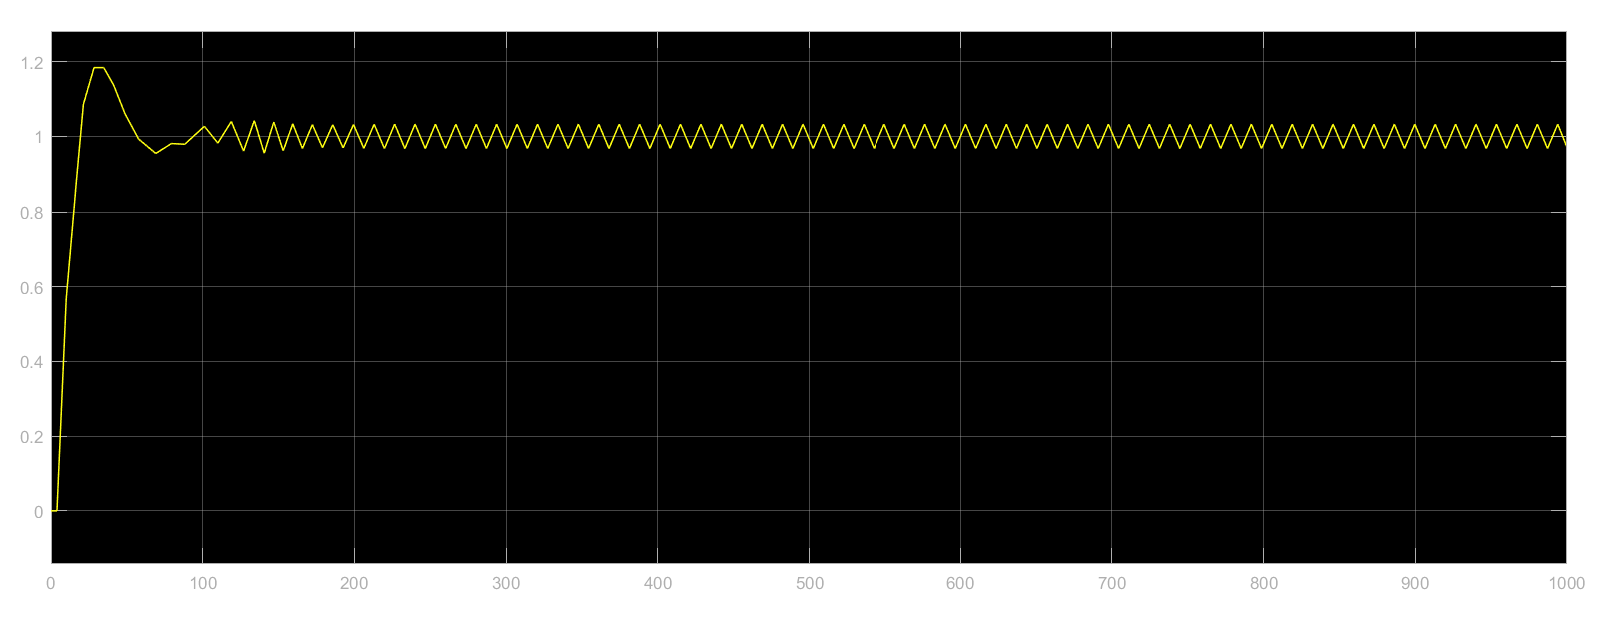
\includegraphics[scale=.50]{ap02810}
\caption{Az $A_P=0.2810$ rendszer ugrásválasza}
\end{figure}
A rendszer a stabilitás határán van továbbra is, így az $A_P$ értékét $A_P=0,2530$-ra csökkentem.
\begin{figure}[H]
\centering
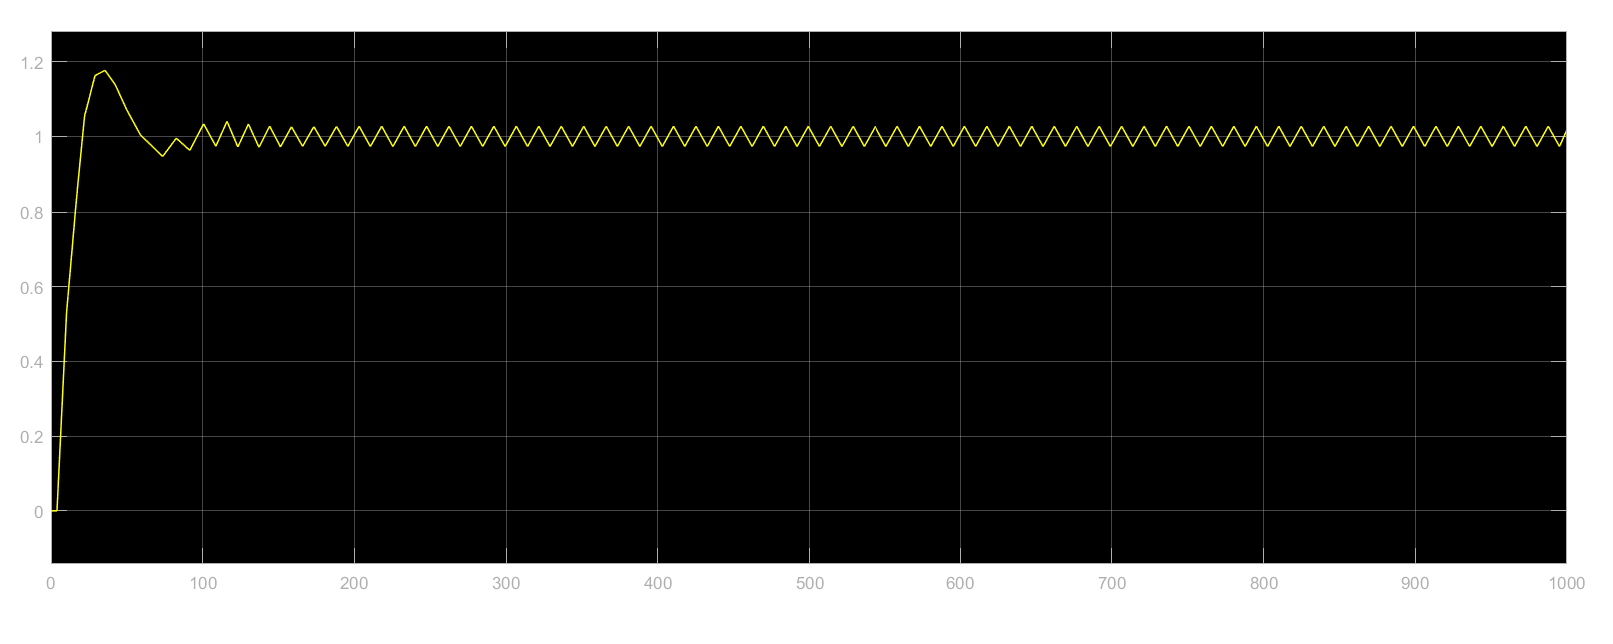
\includegraphics[scale=.50]{ap0253}
\caption{Az $A_P=0.2530$ rendszer ugrásválasza}
\end{figure}
A rendszer továbbra is stabilitás az határán, így az $A_P$ értékét $A_P=0.2390$-re csökkentem.
\begin{figure}[H]
\centering
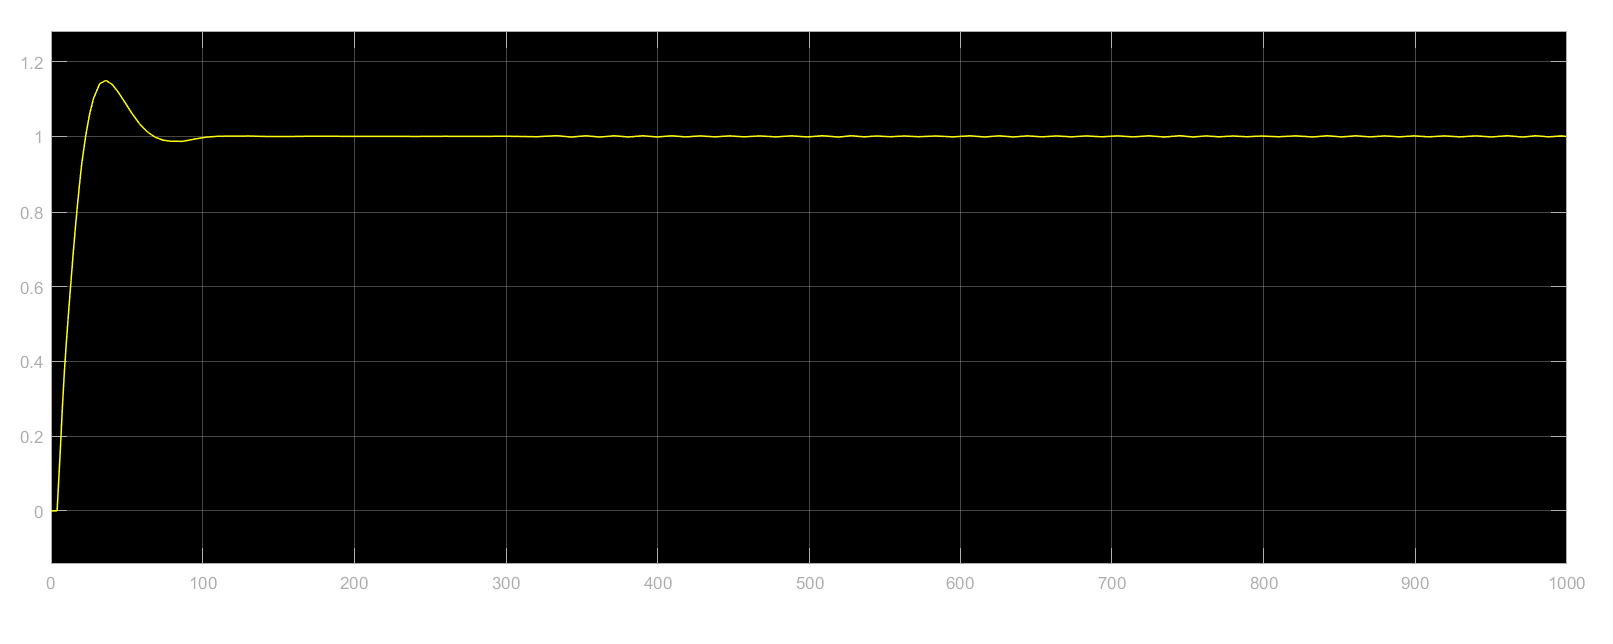
\includegraphics[scale=.50]{ap0239}
\caption{Az $A_P=0.2390$ rendszer ugrásválasza}
\end{figure}
A rendszer stabil így az $AP_P$ értékét $A_P=0.2460$-re növelem.
\begin{figure}[H]
\centering
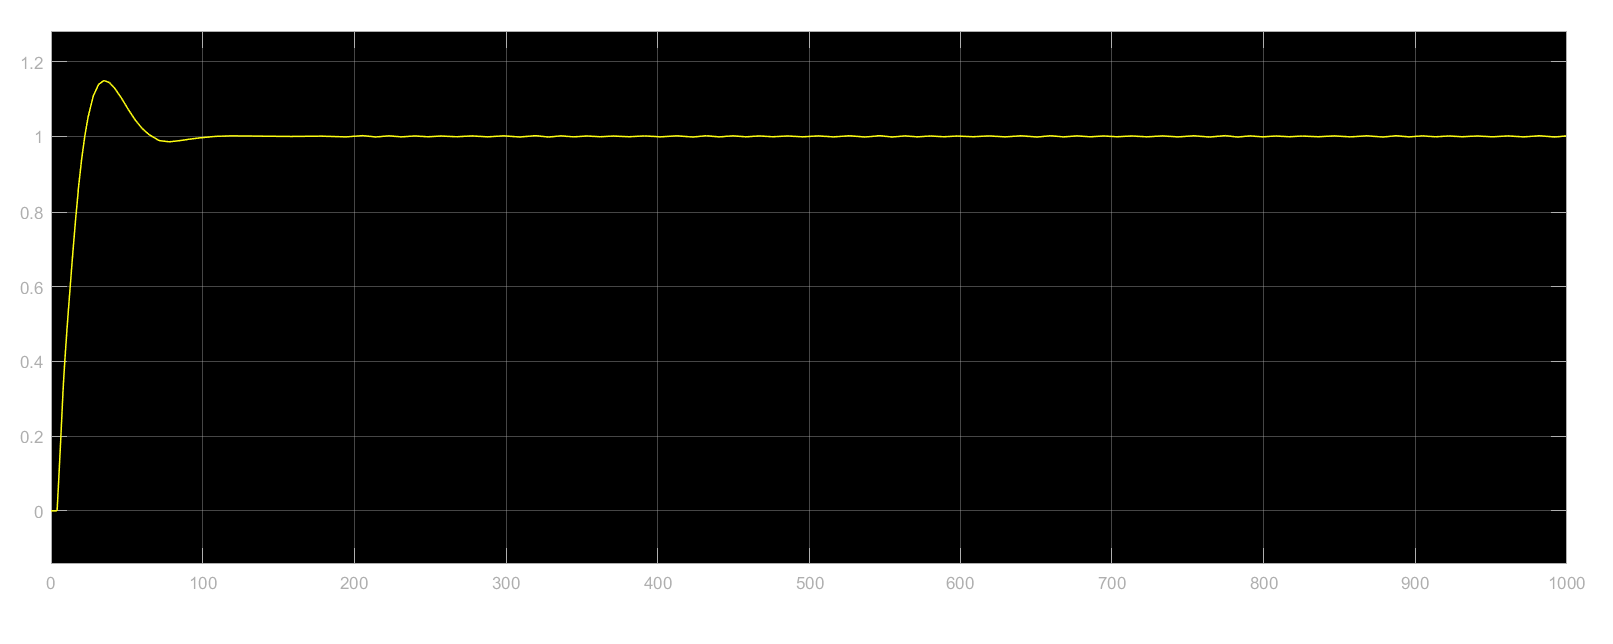
\includegraphics[scale=.50]{ap0246}
\caption{Az $A_P=0.2460$ rendszer ugrásválasza}
\end{figure}
A rendszer stabil így az $A_P$ értékét $A_P=0,2500$-re növelem.
\begin{figure}[H]
\centering
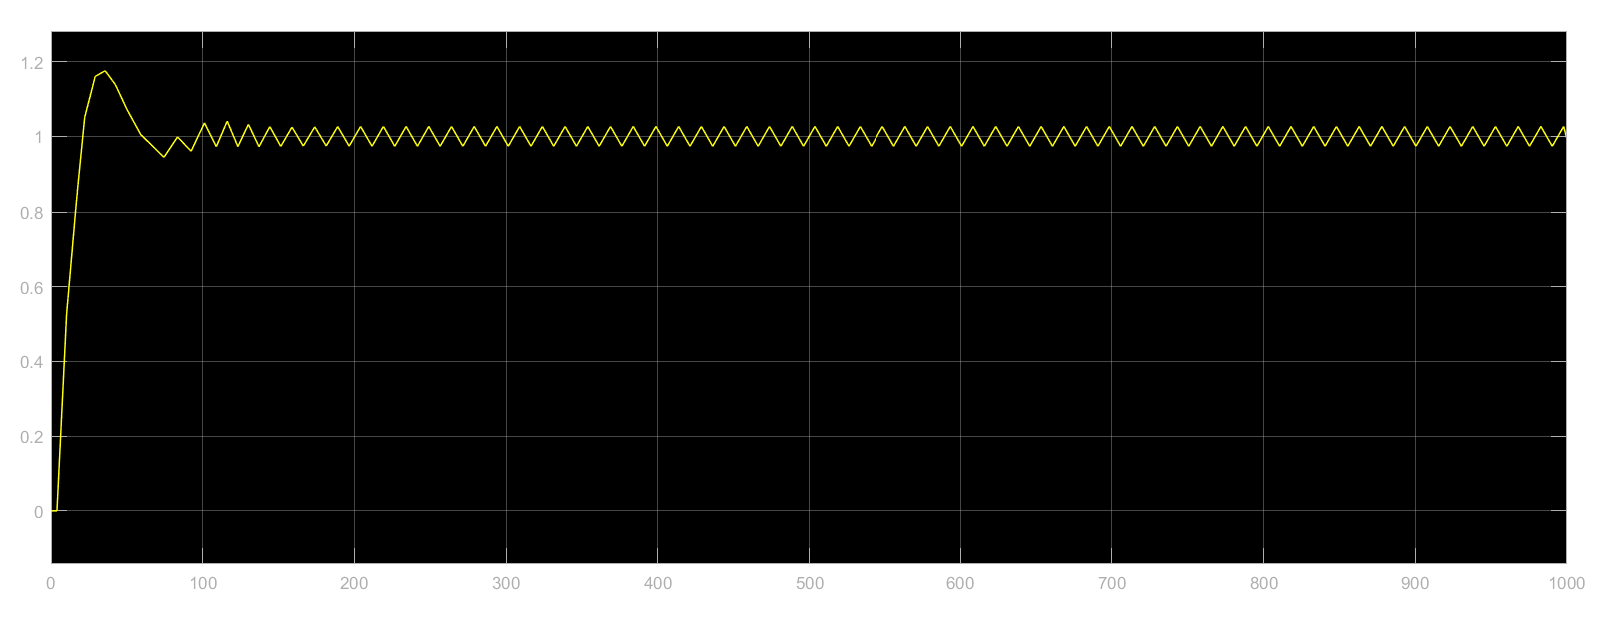
\includegraphics[scale=.50]{ap02500}
\caption{Az $A_P=0.2500$ rendszer ugrásválasza}
\end{figure}
A rendszer a stabilitás határán van, így az $A_P$ értékét $A_P=2482$-re csökkentem.
\begin{figure}[H]
\centering
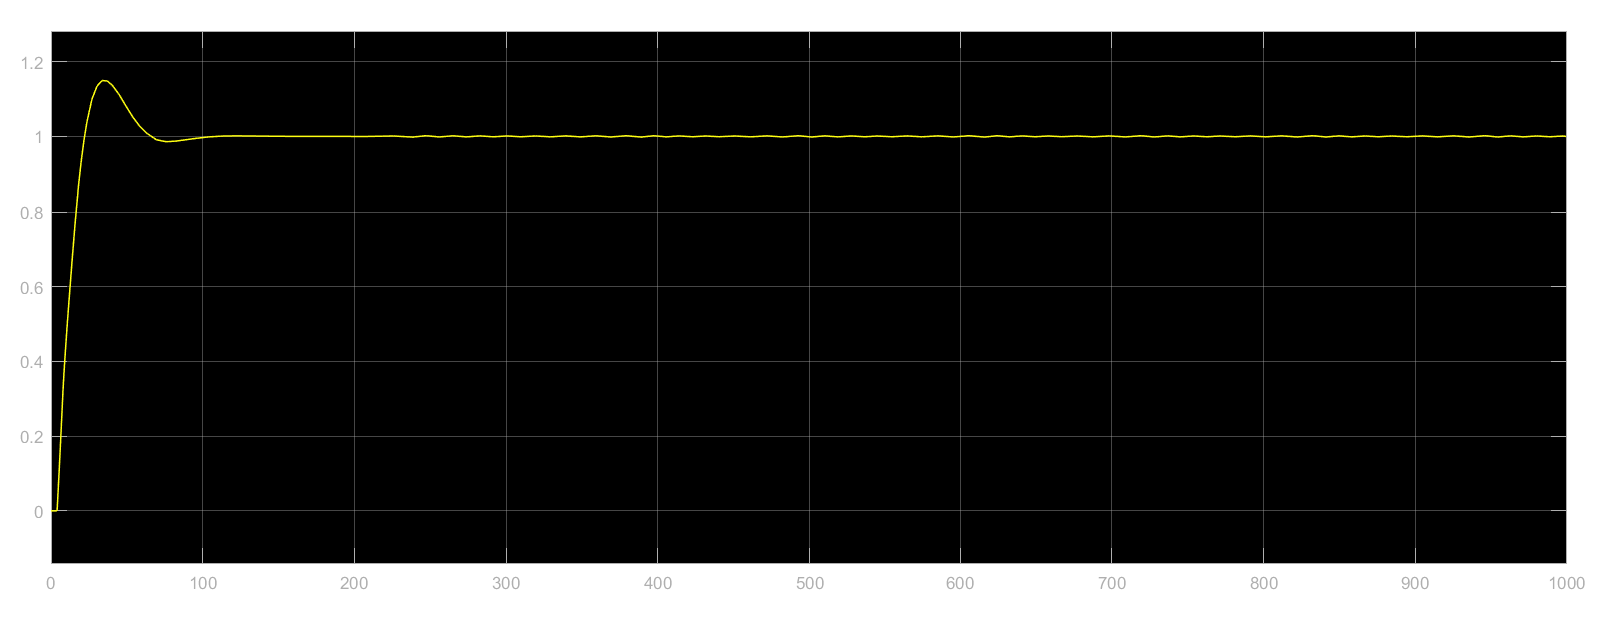
\includegraphics[scale=.50]{ap02482}
\caption{Az $A_P=0.2482$ rendszer ugrásválasza}
\end{figure}
A rendszer stabil, így 3 tizedesjegy pontosságra térve, az $A_P$ erősítést $A_P=.0249$ értékre növeltem, mivel látható, hogy $A_P=0.250$ estén már a stabilitás határán van a rendszer.
\begin{figure}[H]
\centering
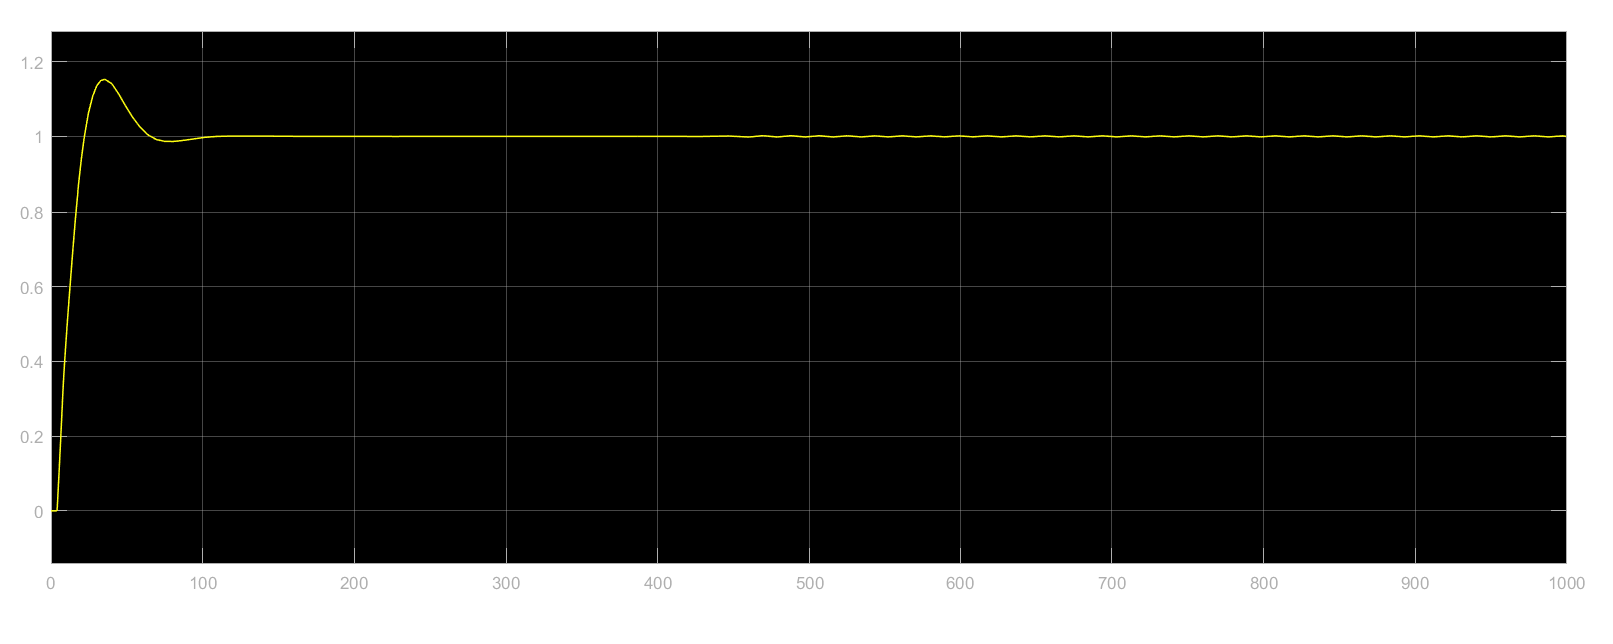
\includegraphics[scale=.50]{ap0249}
\caption{Az $A_P=0.249$ rendszer ugrásválasza}
\end{figure}
A rendszer stabil, van egy túllövése, majd egy alul lövést követve beáll a rendszer állandósult állapotba. A mérések alapján kijelenthető, hogy $A_P=0.249$ erősítésig lehet a rendszert erősíteni.

\subsection{PI szabályozó tervezés Ziegler-Nichols stabilitás határának elérésén alapuló szabályozás módszerével}
Adott átviteli függvény:
\[W_p(s)=\frac{1}{(1+12.4s)(1+5s)(1+1.3s)}e^{-T_us}\]
ahol $T_us=3$
A rendszer tartalmaz késleltetést $T_us=3$, amit Simulink alatt összeállítottam, ahol az stabilitás határának eléréséig egy $K_u$ erősítési a tényezővel állítottam.
\begin{figure}[H]
\centering
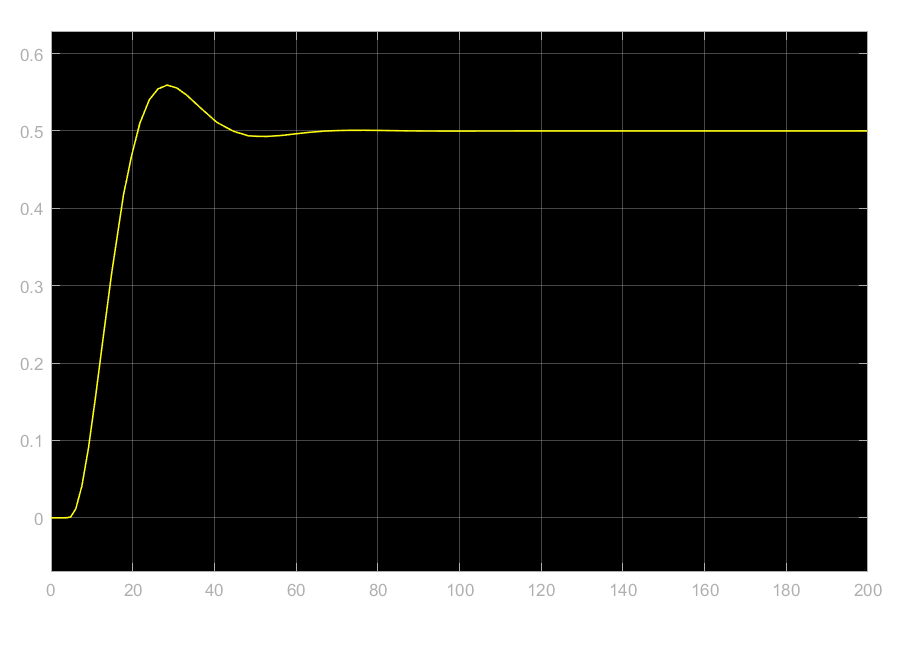
\includegraphics[scale=.70]{ZNSKU1}
\caption{Az $K_u=1$ erősítési tényezővel, a rendszer ugrásválasza}
\end{figure}
$K_u=1$ esetén, a rendszer stabilnak tűnik. Van túllövés, illetve azt követi egy alul lövés, majd beáll állandósult állapotba. Ez alapján véletlenszerűen, empirikus módon az erősítést növeltem $K_u=5$-re.
\begin{figure}[H]
\centering
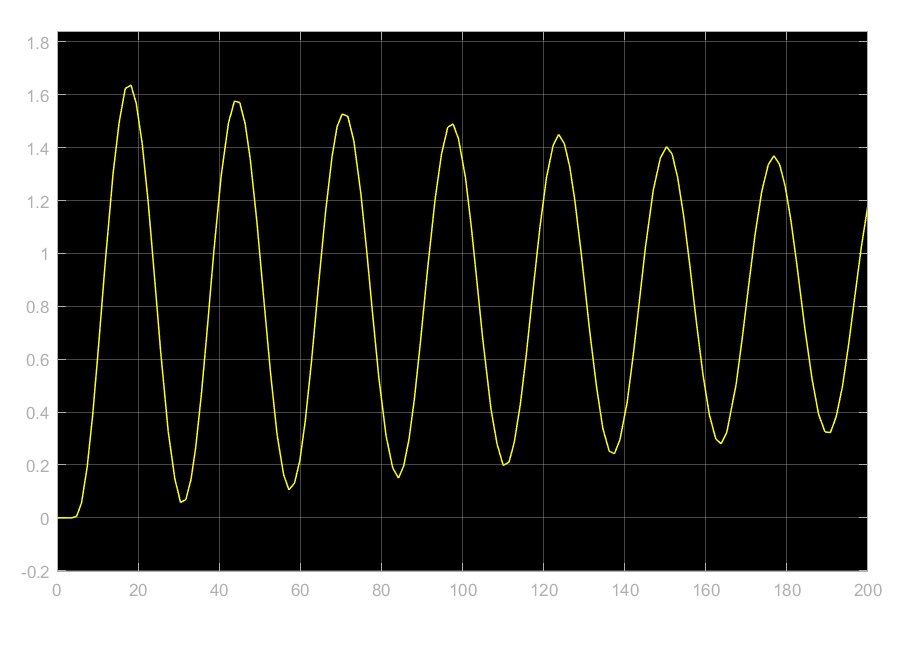
\includegraphics[scale=.70]{ZNSKU5}
\caption{Az $K_u=5$ erősítési tényezővel, a rendszer ugrásválasza}
\end{figure}
A rendszer itt már beleng, a stabilitás határán van. Viszont lehet látni, hogy kezd csillapodni. Az erősítést $K_u=5.5$-re tovább emelem.
\begin{figure}[H]
\centering
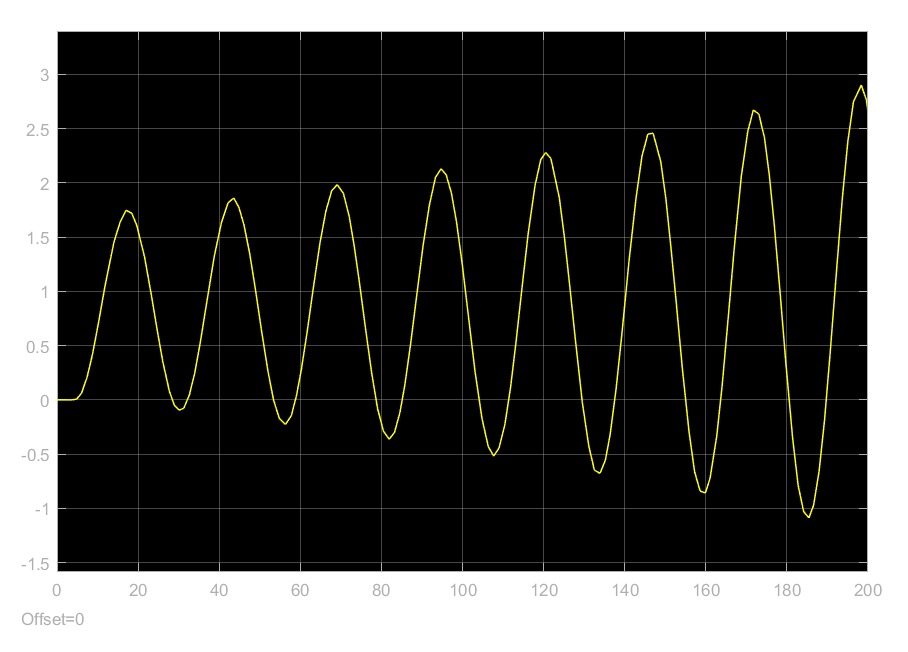
\includegraphics[scale=.70]{ZNSKU55}
\caption{Az $K_u=5.5$ erősítési tényezővel, a rendszer ugrásválasza}
\end{figure}
A rendszer instabil, így az optimális erősítés $5<K_u<5.5$ helyen található. Empirikus próbálkozások után $K_u=5.167$ esetén van a stabilitás határán.
\begin{figure}[H]
\centering
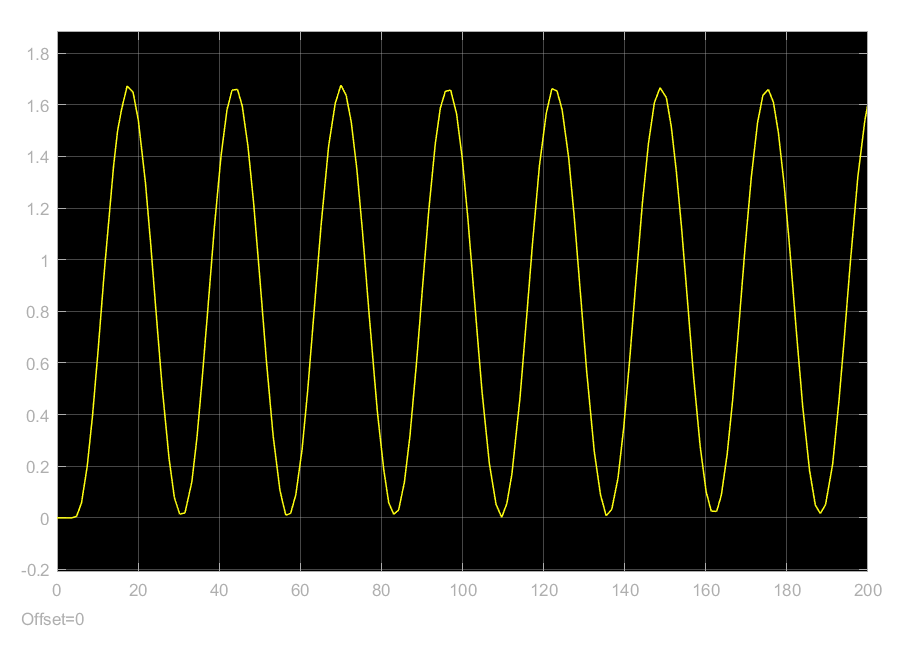
\includegraphics[scale=.70]{ZNSKU5167}
\caption{Az $K_u=5.167$ erősítési tényezővel, a rendszer ugrásválasza}
\end{figure}
Az ugrásválasz alapján leolvasom a két közeli kilengési ponton a periódus időt, ami $P_u=26.174$.
\begin{figure}[H]
\centering
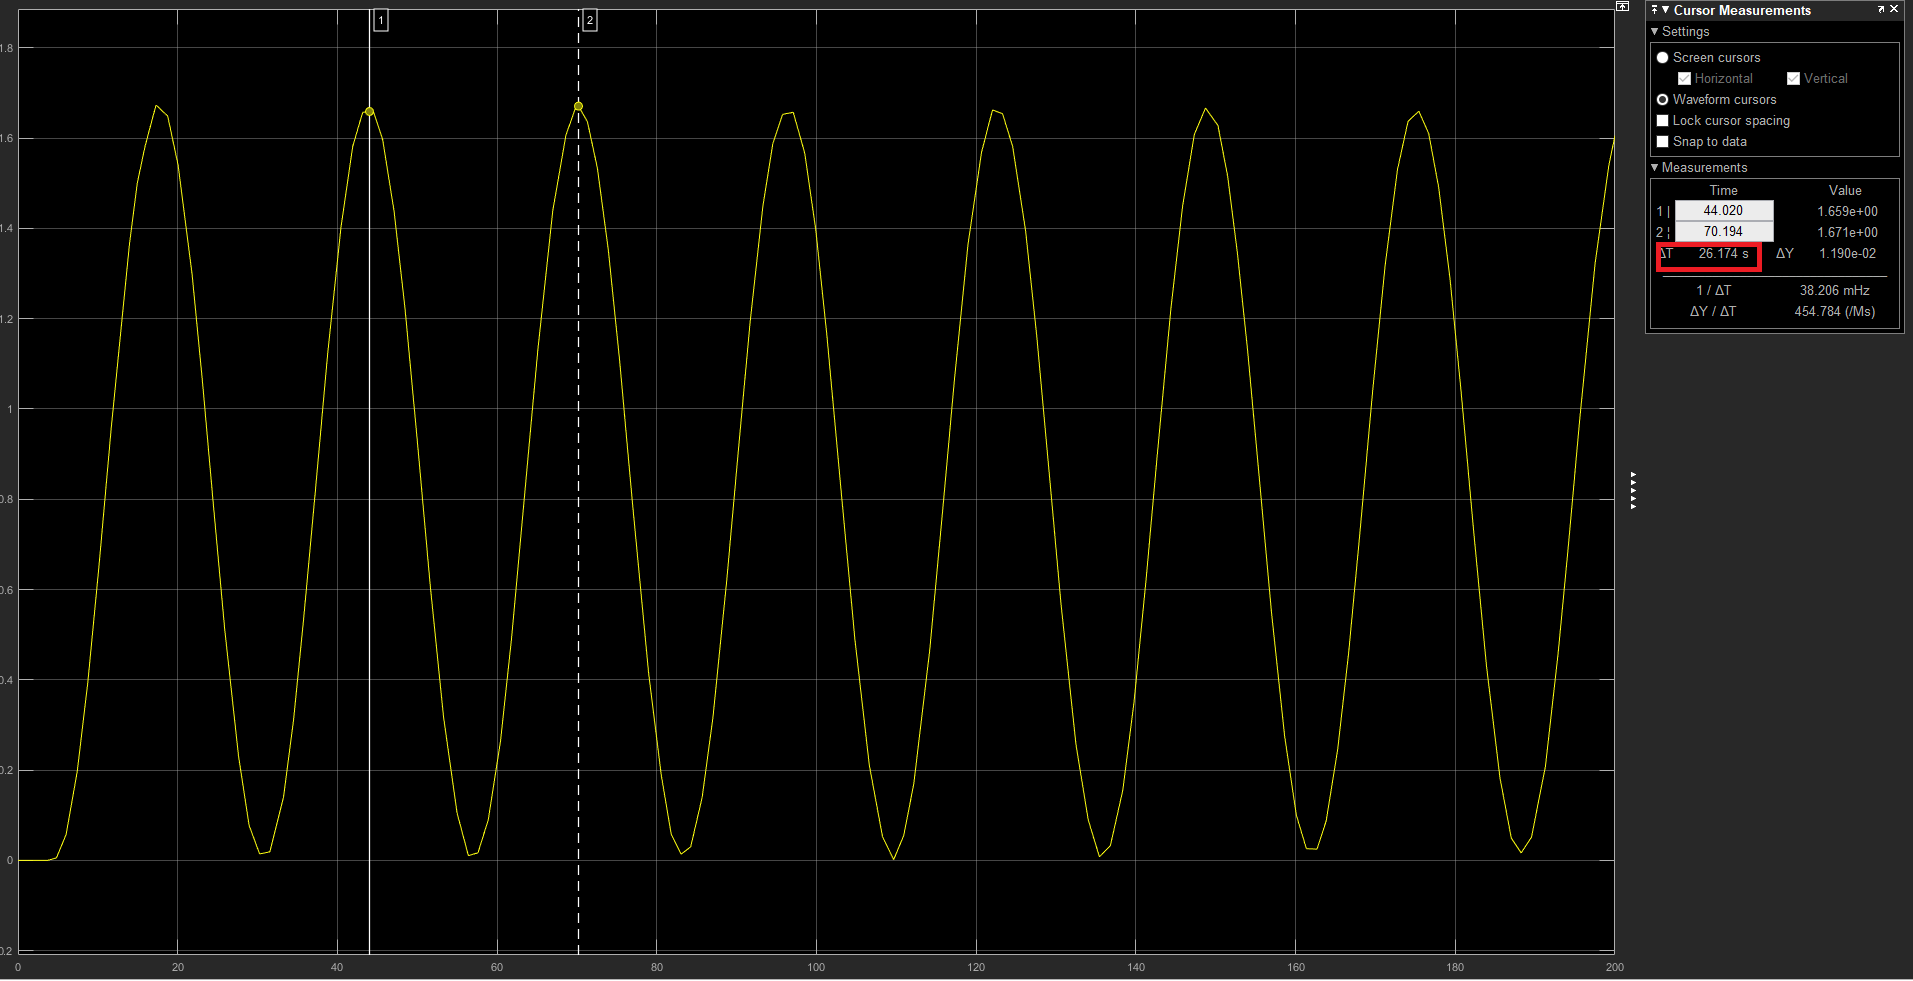
\includegraphics[scale=.30]{ZNSKPERIOD}
\caption{Az ugrásválaszból leolvasott $P_u=26.174$ periódus idő}
\end{figure}
PI szabályozó esetén így ki tudjuk számolni a 
\[A_p=0.45*K_u=0.45*5.167=2.325 \]
\[T_I=0.85*P_u=0.85*26.174=22.247 \]
A PI szabályozó átviteli függvénye:
\[WPI=A_p*(1+\frac{1}{sT_I})=2.325*(1+\frac{1}{22.247s})=\frac{51.73s+2.325}{22.25s}\]
A PI szabályozó átviteli függvényét elhelyeztem Simulink kapcsolásba az erősítés helyére.
Az ugrásválasz:
\begin{figure}[H]
\centering
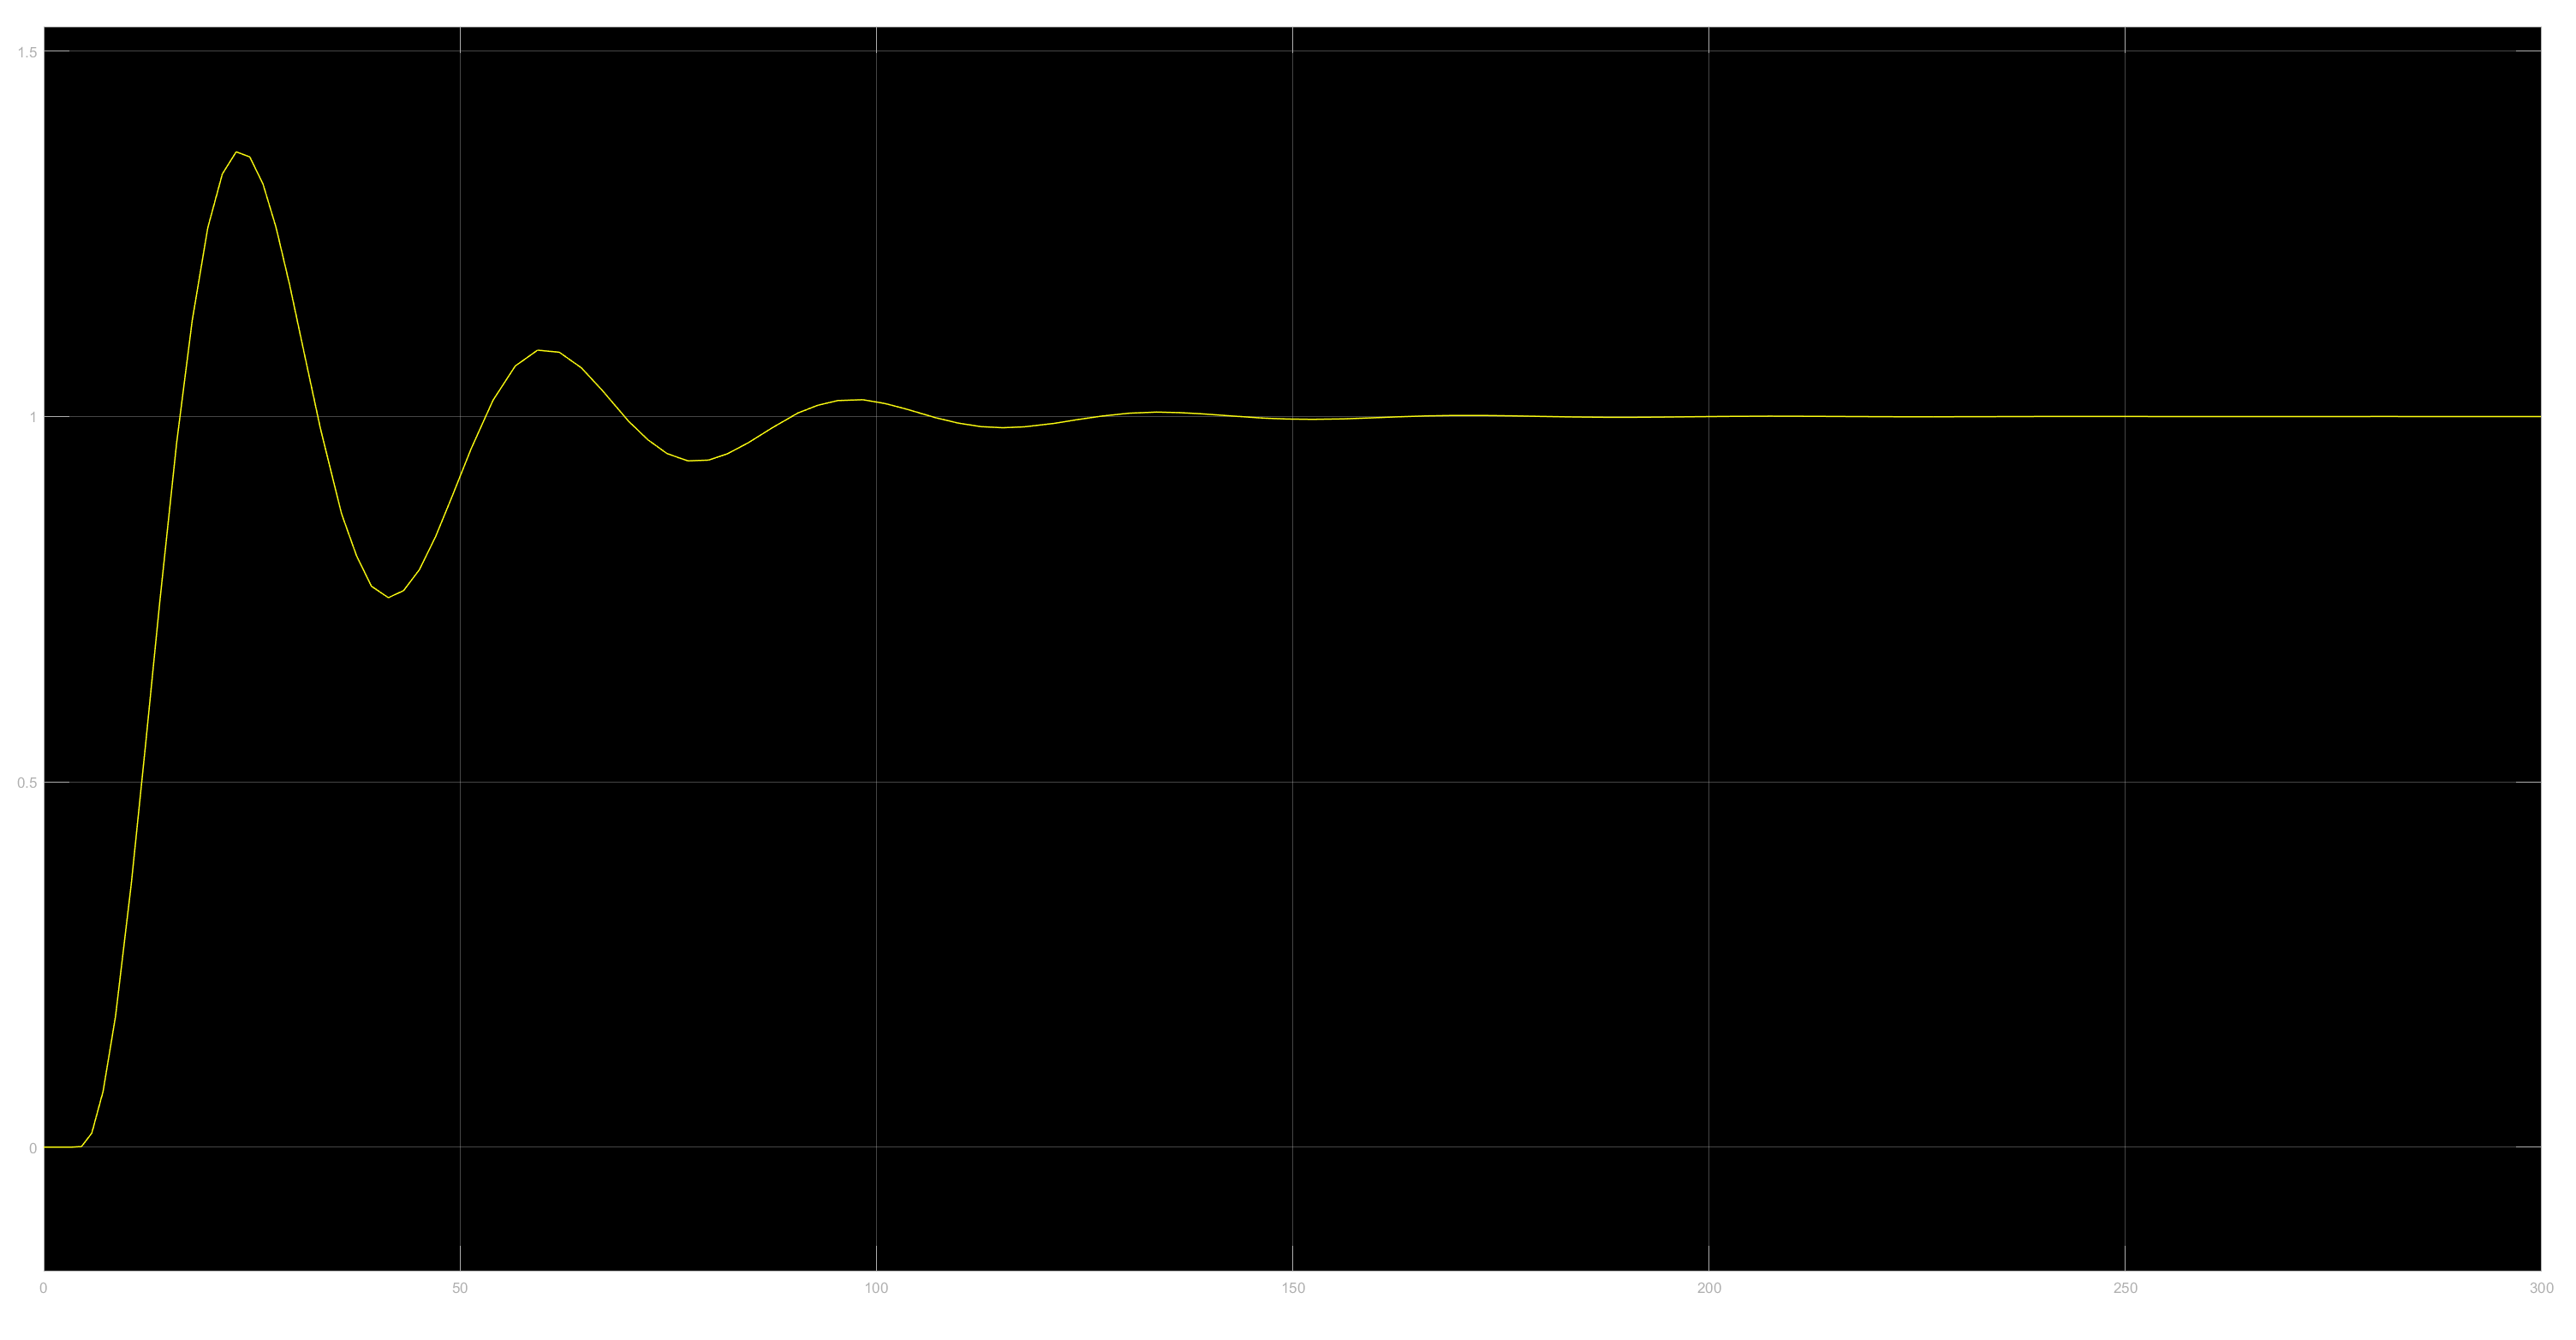
\includegraphics[scale=.30]{ZNSKUPI}
\caption{A tervezett PI szabályozóval, a rendszer ugrásválasza}
\end{figure}
A rendszer stabil, 1-re áll be a szabályozó, előtte van túllövése 1,3 majd 1,1 környékén. Végül 150-nél beáll a rendszer.

\subsection{PID szabályozó tervezés Kessler módszerrel}
Adott átviteli függvény:
\[W_p(s)=\frac{1}{(1+12.4s)(1+5s)(1+1.3s)}e^{-T_us}\]
ahol $T_us=0$
A rendszer nem tartalmaz holtidőt, mivel a $T_U=0$, illetve nem tartalmaz szabad integrátort (nincs s-el való szorzás a pólusok elején), így a modulusz kritériumot fogom használni. A rendszer Matlab-ba betöltöttem. PID szabályozó esetén a szabályozandó rendszernek \[W_p(s)=\frac{K_P}{(1+1s*T_1)(1+s*T_2)(1+s*T_3)}\] alakúnak kell lennie. A rendszer jelenleg ilyen alakúnak néz ki, így nem kell alkalmazni a kis időállandó tételét.\begin{center}
\begin{tabular}{| c c c |}
\hline $T_{r1}$ & $T_1$ & 12.4 \\
\hline $T_{r2}$ & $T_2$ & 5 \\
\hline $T_{\sum}$ & $T_3$ & 1.3 \\
\hline & $K_p$ & 1 \\
\hline
\end{tabular}
\end{center}
A szükséges paraméterek a \[K_r=\frac{1}{2*K_p*T_\sum}=\frac{1}{2*1*1.3}=0.3846\] 
A PID szabályozó átviteli függvénye: \[\frac{K_r}{s}*(1+sT_{r1})(1+sT_{r2})\]
A Matlab által kiszámolt PID szabályozó átviteli függvény: \[W_{PID}(s)=\frac{23.85s^2+4.769s+0.3846}{s}\]
Ezt Simulink alatt nem lehet felvinni, mint átviteli függvény, ezért ki kell számolni külön a P I D tagok átviteli függvényét, ami:
\[(1+s*T_1)*(1+sT_2)=62s^2+17.4s+1\]
Ebből a tagok külön:
\begin{center}
\begin{tabular}{|c c c|}
\hline P & $\frac{K_r}{s}*17.4*s$ & 6.692 \\
\hline I & $\frac{K_r}{s}*1$ & $\frac{0.3846}{s}$\\
\hline D & $\frac{K_r}{s}*62*s^2$ & $23.85s$\\
\hline
\end{tabular}
\end{center}
A Simulink segítségével összerakott rendszer ugrásválasza
\begin{figure}[H]
\centering
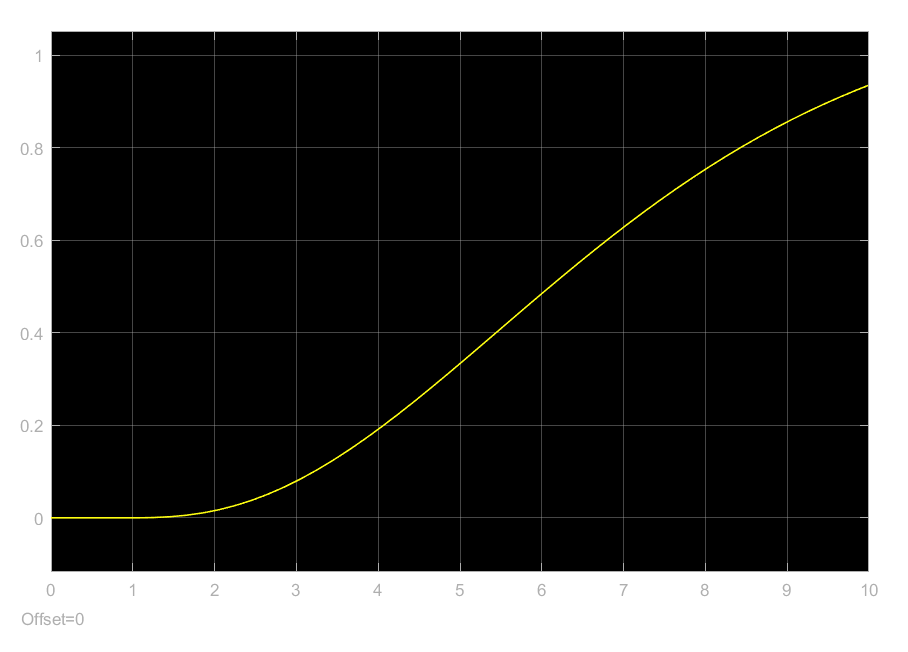
\includegraphics[scale=.70]{KESSLER10S}
\caption{A rendszer ugrásválasza $10s$ szimulációs idővel}
\end{figure}
A rendszer nem tűnik stabilnak, azonban gyanú lehet egy túllövés, ezért a szimulációs időt megemeltem.
\begin{figure}[H]
\centering
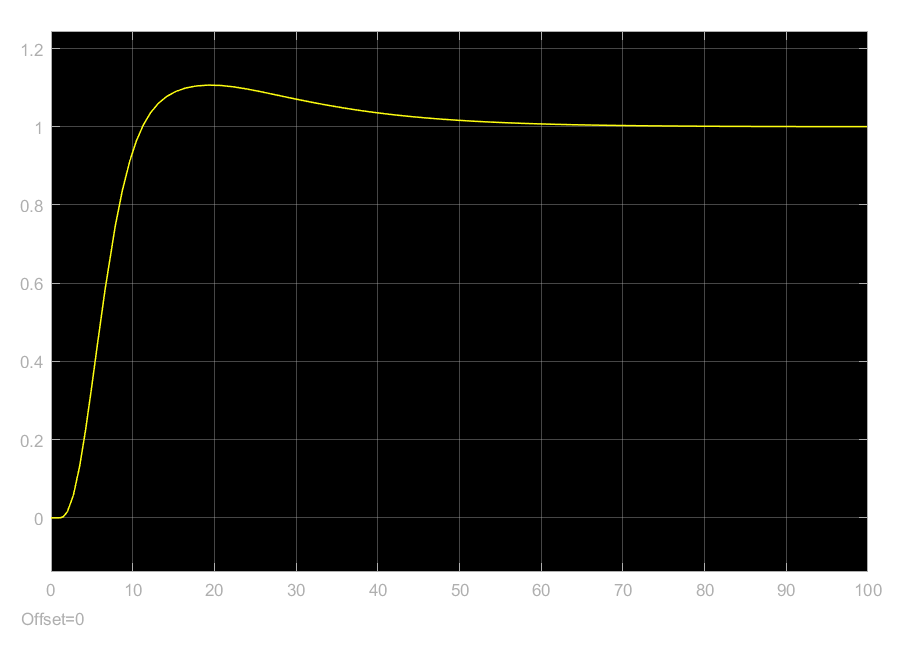
\includegraphics[scale=.70]{KESSLER100S}
\caption{A rendszer ugrásválasza $100s$ szimulációs idővel}
\end{figure}
A rendszer stabil, ahogy az ábrán látható, hogy a rendszernek van $1.343s$ holtideje, amit egy, majd kb $16.864s$ múlva eléri a túllövés maximumát, ami a $18.207s$-nél történik. Majd $51.780s$ múlva $69.800s$-nél beáll 1-re, azaz az állandósult állapotra.
\section{Klasszikus PID szabályozó tervezés}
A szabályozandó szakasz: \[W_P(s)=\frac{1}{(1+12.4s)(1+5s)(1+1.3s)}\]
A szabályozandó szakasz a szorzások elvégzése után, amivel dolgozni fogok:
\[W_P(s)=\frac{1}{80.6s^3+84.62s^2+18.7s+1}\]
Bármilyen szabályozó tervezésnek nekiállok, megnézem a rendszer ugrásválaszát:
\begin{figure}[H]
\centering
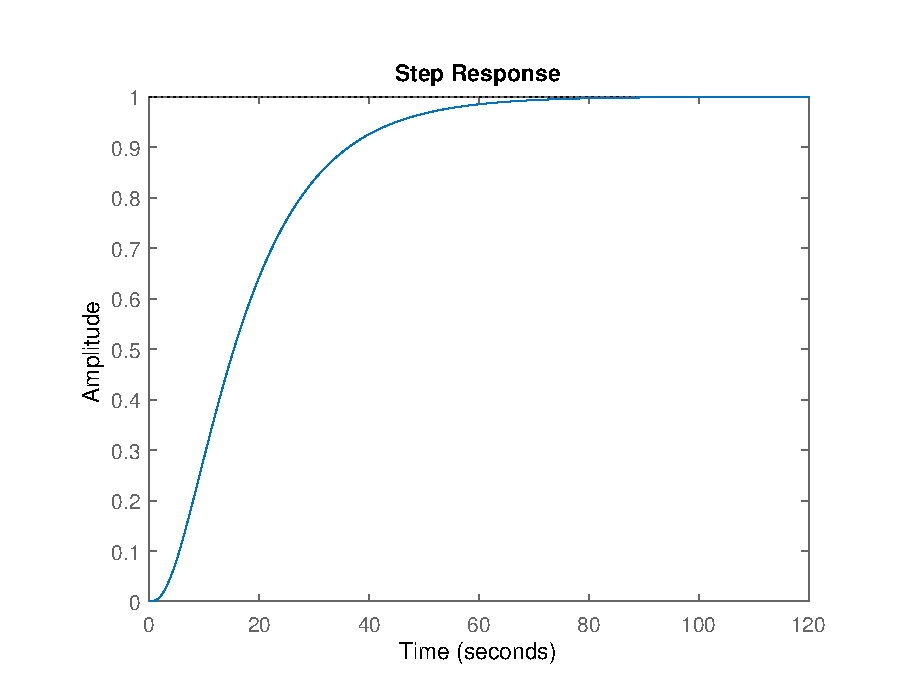
\includegraphics[scale=.70]{WPLANTSTEPRESPONSE}
\caption(A szabályozandó rendszer ugrásválasza)
\end{figure}
A rendszer stabil, kb $80s$-nél beáll 1 állandósult állapotba. Nincs túllövése, csak felfutási ideje. 
\begin{figure}[H]
\centering
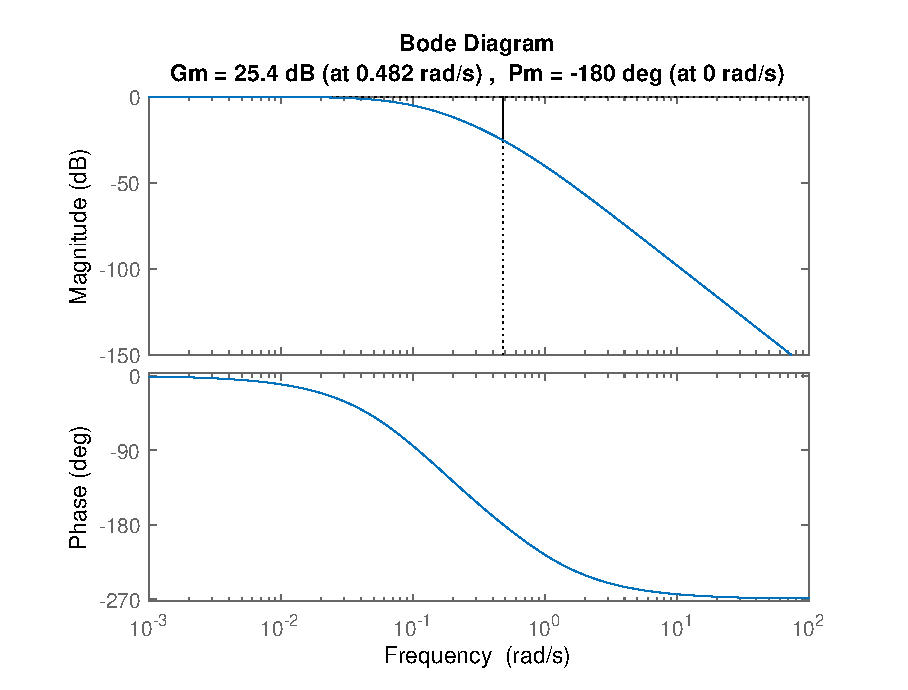
\includegraphics[scale=.70]{WPLANTMARGIN}
\caption(A szabályozandó rendszer Bode diagramja)
\end{figure}
A Bode diagramon látható, hogy a Fázistartalék $\varphi_t=-180^\circ$ az erősítés pedig $25.4dB$
\subsection{P szabályozó tervezés $\varphi_t=70^\circ$ fázistartalékra}
A szabályozó tervezés első lépése, hogy egy $\frac{1}{1}$-es szabályzót hozok létre, amit sorba kötök a rendszerrel. Ezt elsőként nyitott körre hajtom végre. A kiértékelést numerikus módszerrel hajtom végre. A $70\circ$ tartalékot Matlab-ban eltároltam, majd a Bode diagramból eltároltam az amplitudókat, a fázisokat, és a $\omega$-kat. Ezek után kiszámoltam az abszolút távolságokat  $\varphi_t=70^\circ$-től az alábbi módon:
$(180^\circ+phases)-70^\circ$ abszolút értéke, majd vettem ennek a listának a minimumát. A minimum indexű fázisból kinyertem az erősítési tényezőt $A_P=2.5808$. A P szabályozó $\frac{A_P}{1}$, melyet sorba kötve megkaptam a nyitott kör Bode diagramját:
\begin{figure}[H]
\centering
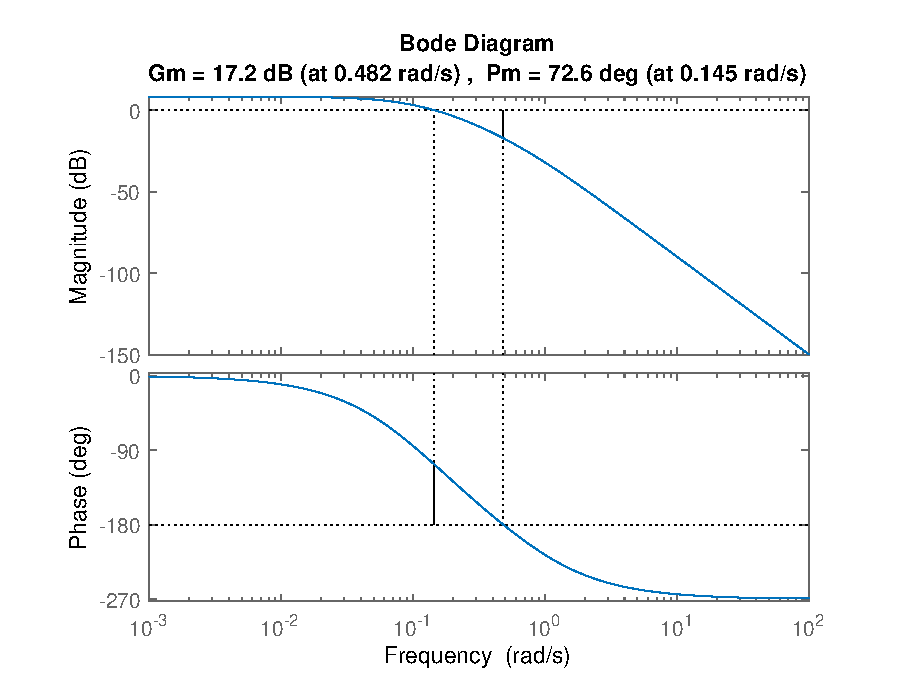
\includegraphics[scale=.70]{WPLANTPIDOPENLOOPMARGIN}
\caption(A P szabályozóra tervezett nyitott kör Bode diagramja)
\end{figure}
A diagram alapján látható, hogy a numerikusan módszerrel tervezett fázistartalék $72.6^\circ$ lett, ami annak köszönhető, hogy a Matlab bode függvénye az amplitúdó és fázisdiagramot diszkrét frekvenciaértékeken értékeli ki. A zárt rendszert létrehozásához egy hurok visszacsatoló ágat létrehozva a zárt köt ugrásválasza:
\begin{figure}[H]
\centering
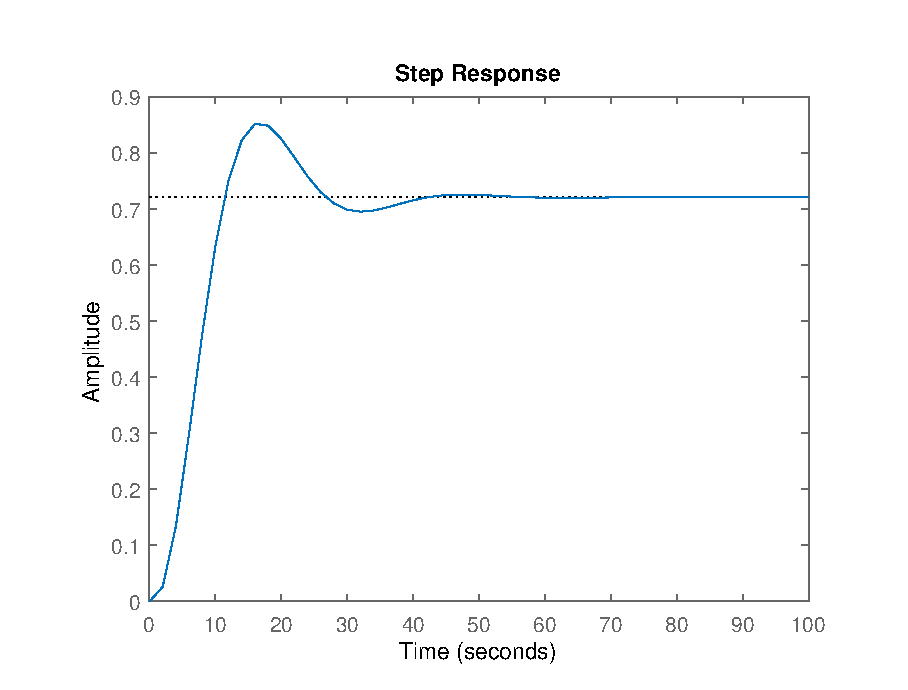
\includegraphics[scale=.70]{WPLANTPCLMR}
\caption(A P szabályozóra tervezett zárt kör ugrásválasza)
\end{figure}
A rendszer továbbra is stabil, illetve egy túllövése 0.87 amplitudó környékén, majd beáll a 0.72 amplitudó környékén.
\subsection{P szabályozó tervezés előírt állandósult hibára $e=0.1$}
Az állandósult hiba eléréséhez az erősítést kell felhasználni:
\[e=1-\frac{K}{1+K}\Rightarrow K=\frac{1-e}{e}\]
\[K_p*K_{Plant}=\frac{1-e}{e}\]
\[K_p=\frac{1-e}{K_{Plant}*e}\]
Az egyenletbe való helyettesítés után a $K=9$ az erősítés. A szabályozandó rendszer erősítése $K_{Plant}=1$, amelyet a Matlab dcgain függvényéből olvastam ki a szabályozandó rendszerhez. Így szabályozó erősítése $K_P=9$. A nyitott kör P szabályozós átviteli függvénye:
\[W_P(s)=\frac{9}{80.6s^3+84.62s^2+18.7s+1}\]
A nyitott kör Bode diagramja:
\begin{figure}[H]
\centering
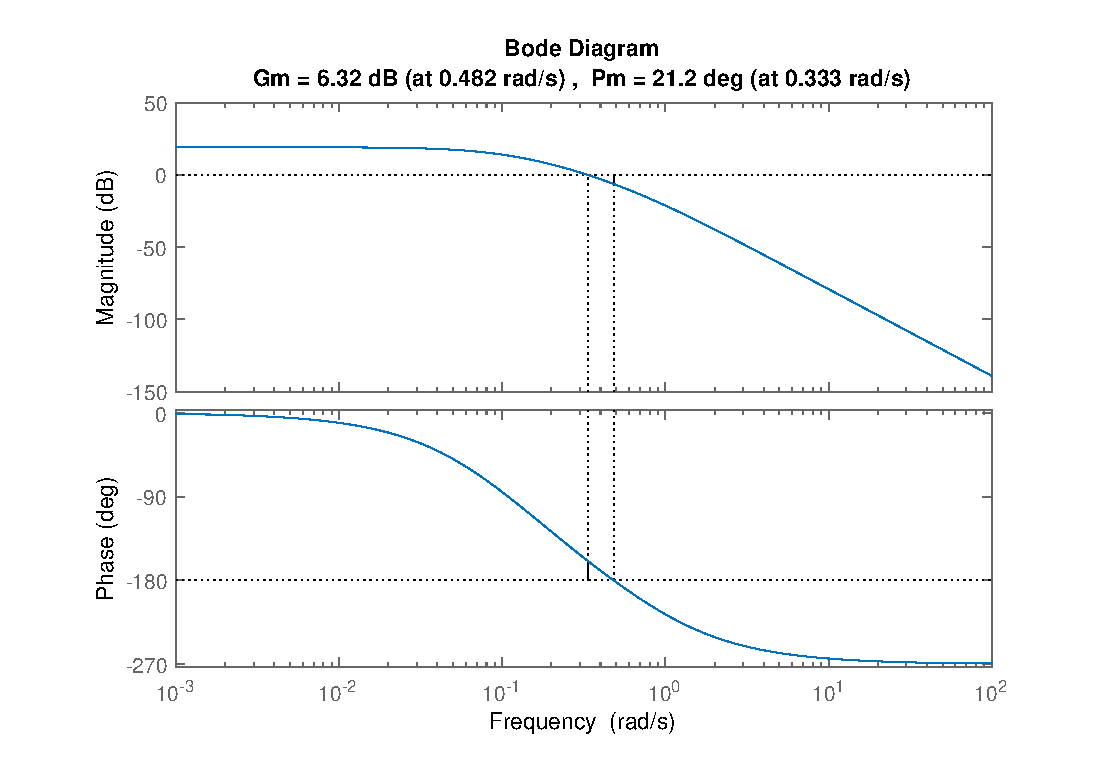
\includegraphics[scale=.70]{WOERRORMARGIN}
\caption(A P szabályozóra tervezett nyitott kör Bode diagramja)
\end{figure}
A Bode diagramm alapján a nyitott kör fázistartaléka $\varphi_t=21.2$ 
A rendszer ugrásválasza:
\begin{figure}[H]
\centering
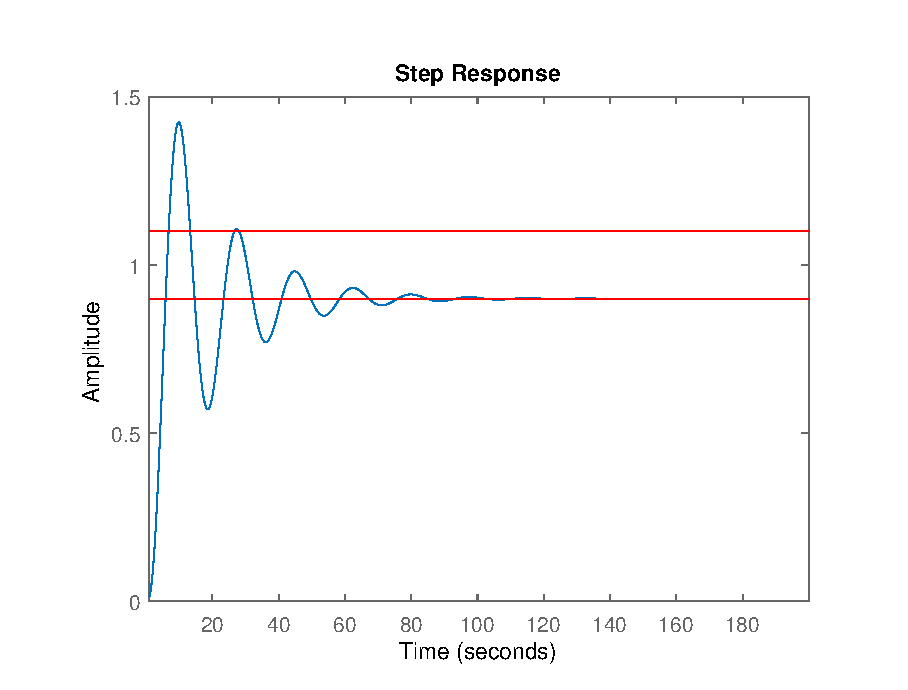
\includegraphics[scale=.70]{WCLOSEDERORSTEP}
\caption(A P szabályozóra tervezett zárt kör ugrásválasza)
\end{figure}
A rendszer stabil, igaz vannak túllövései, de beáll 0.9-re, így látható is, hogy az állandósult az hiba $0,1$ lett.
\subsection{Közelítő PD szabályozó tervezés előírt vágási frekvenciára $\omega c=0.8\frac{rad}{sec}$}
A szabályozó  tervezéséhez az első körben a második leglassabb pólust kiejtettem.
\[T_D=\frac{T2}{1.1}=\frac{5}{1.1}=0.4545\]
\[T_C=0.1*T_D=0.1*0.4545=4.5455\]
Ellenőrzésképpen a $T_D+TC=5$ ezért nem rontottam el semmit. A tervezés folyamata szerint egy előszabályozót tervezek $A_P=1$ értékkel, de az $A_P$ értéke így is $1$ akár lehetne ez is a szabályozó. Az előszabályozóval létrehozott nyitott kör átviteli függvénye:
\[W(s)=\frac{5s+1}{36.64s^4+119.1s^3+93.12s^2+19.15s+1}\]
Ezt követően a kiszámoltam a amplitudó és fázis értékeke a $\omega c$ vágási frekvencián. Ehhez a matlab függvényt használtam fel, ahol az amplitudó $mag=0.0653$ és a frekvencia $phase=-150.3501$. Végül az $Ap=\frac{1}{mag}=\frac{1}{0.653}=15.3064$. Végül a nyitott kör átviteli függvénye:
\[W(s)=\frac{76.53s+15.31}{36.64s^4+119.1s^3+93.12s^2+19.15s+1}\]
\begin{figure}[H]
\centering
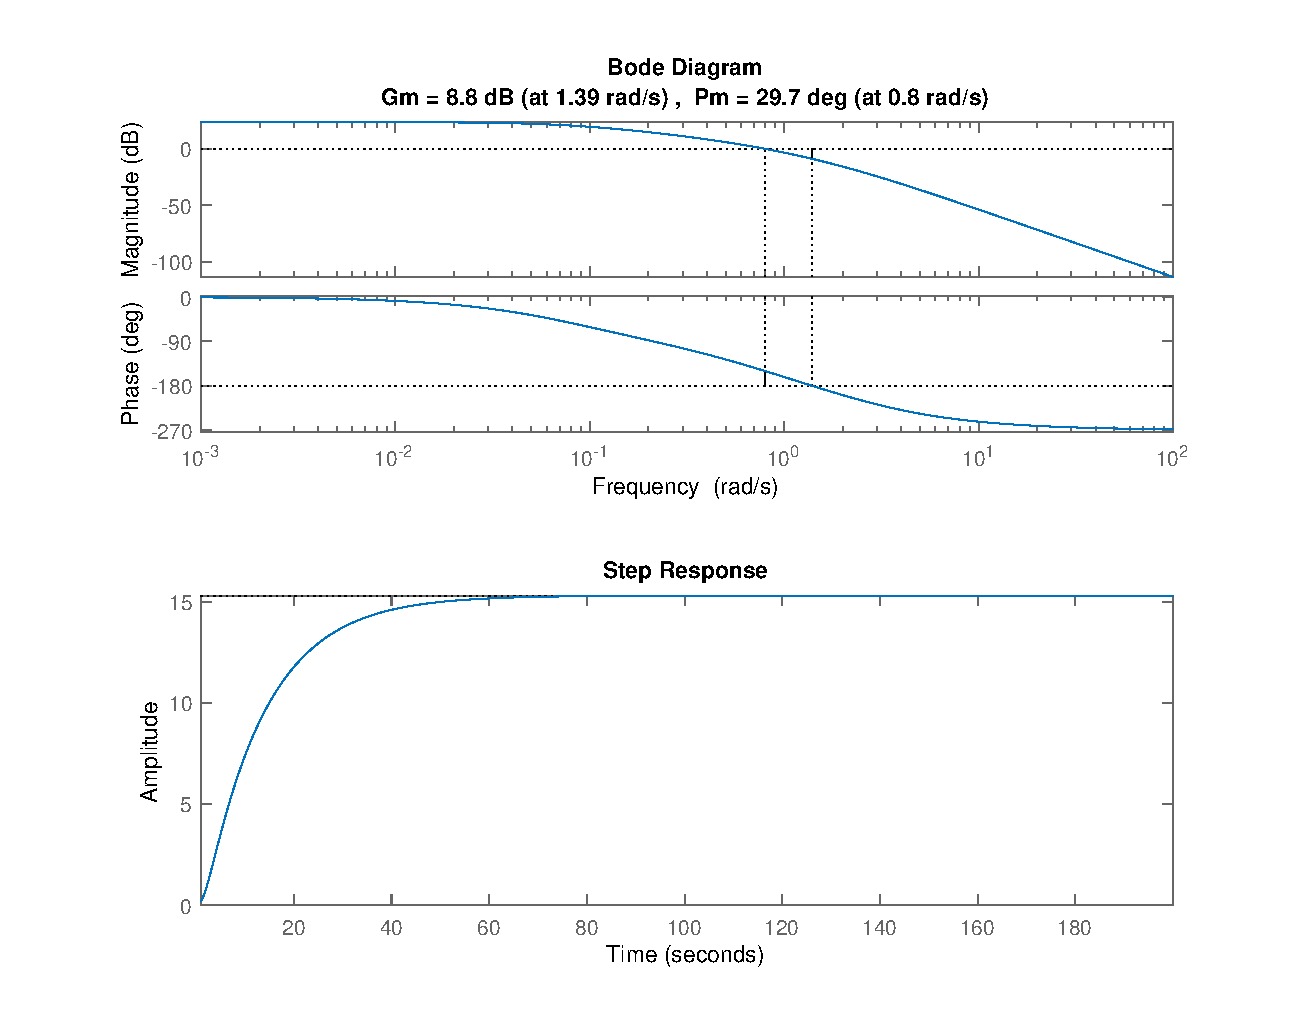
\includegraphics[scale=.70]{WPDOPEN}
\caption(A PD szabályozóra tervezett nyitott kör Bode digramja és ugrásválasza)
\end{figure}
Az ábra alapján látható, hogy a pontosan $0.8\frac{rad}{sec}$ a vágási frekvencia és az ugrásválasz alapján a rendszer stabil, ami 15 amplitudóra áll be. Hibajel nincs.
A zárt kör:
\begin{figure}[H]
\centering
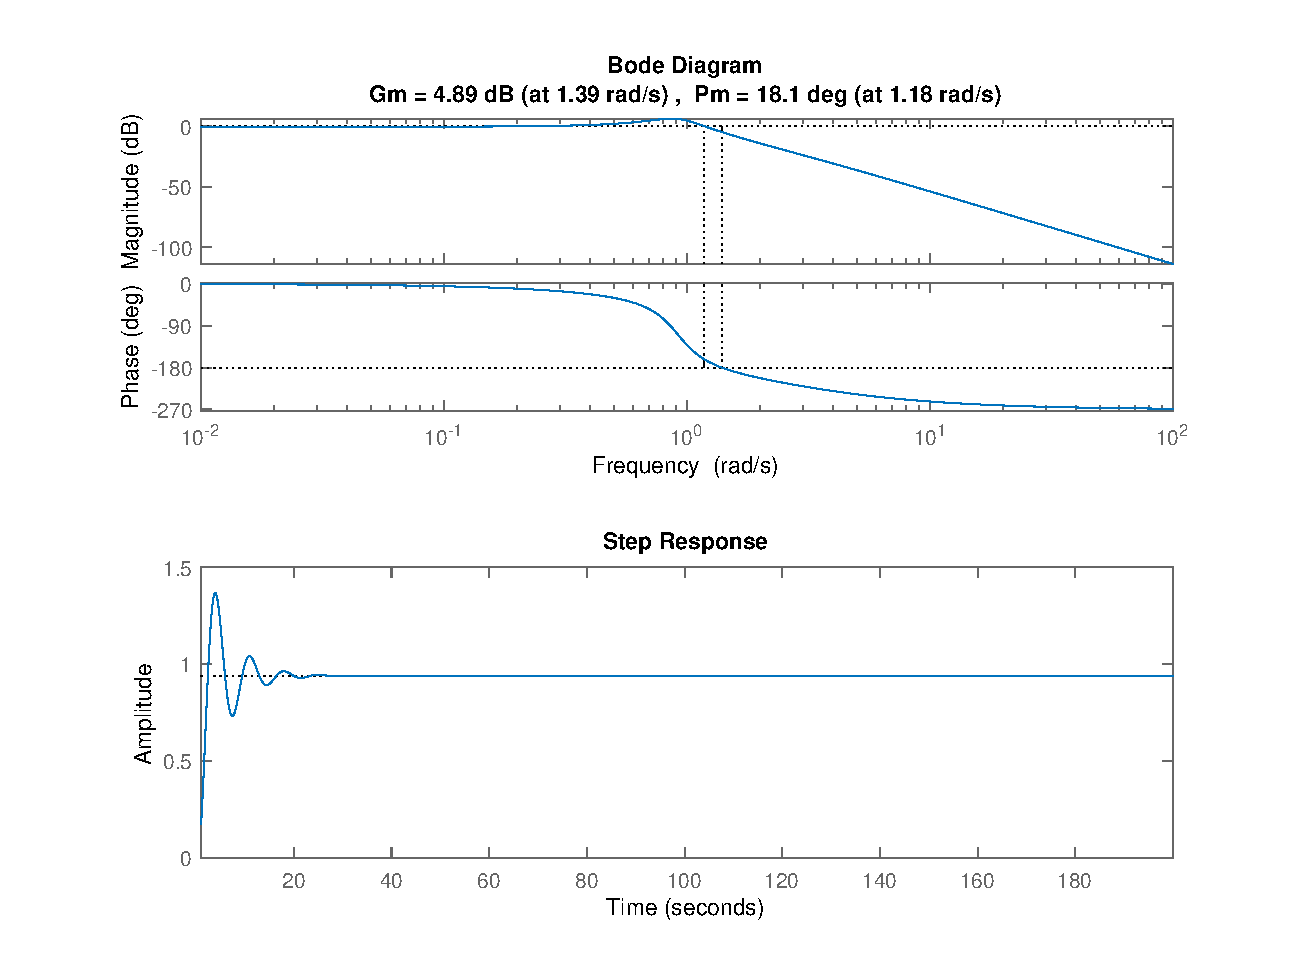
\includegraphics[scale=.70]{WCLOSED_PD}
\caption(A PD szabályozóra tervezett zárt kör Bode digramja és ugrásválasza)
\end{figure}
A rendszer itt is stabil, vannak túllövései, majd beáll egyre.
\subsection{PI szabályozó tervezés előírt fázistartalékra $\varphi_t=70^\circ$ és nulla állandósult hibára}
Első körben kiejtem a leglassabb pólust ami $T_I=T_1=12.4$. A PI szabályozó átviteli függvény \[W_{PI}=\frac{A_P}{T_I}*\frac{1+sT_I}{s}\]  ahol egy előszabályozót hozok létre ahol az  $\frac{A_P}{T_I}=1$. Ebből létrehoztam egy nyitott kört a tervezett rendszerre:
\[W(s)=\frac{12.4s+1}{80.6 s^4+84.62s^3+18.7s^2+s}\]
A nyitott körön megkerestem a vágási frekvenciát, ahol a matlab index $26$ és a frekvencia  $0.1751$. Ebből az $A_P$ érték kiszámítása:
\[A_P=\frac{T_I}{mag[phiidx]}=0.7382\]
Az új $A_P$ értéket felhasználva az új rendszer:
\[W(s)=\frac{9.153s +0.7382}{999.4 s^4+1049s^3+231.9s^2+12.4s}\]
A rendszer bode diagramja nyitott kör esetén:
\begin{figure}[H]
\centering
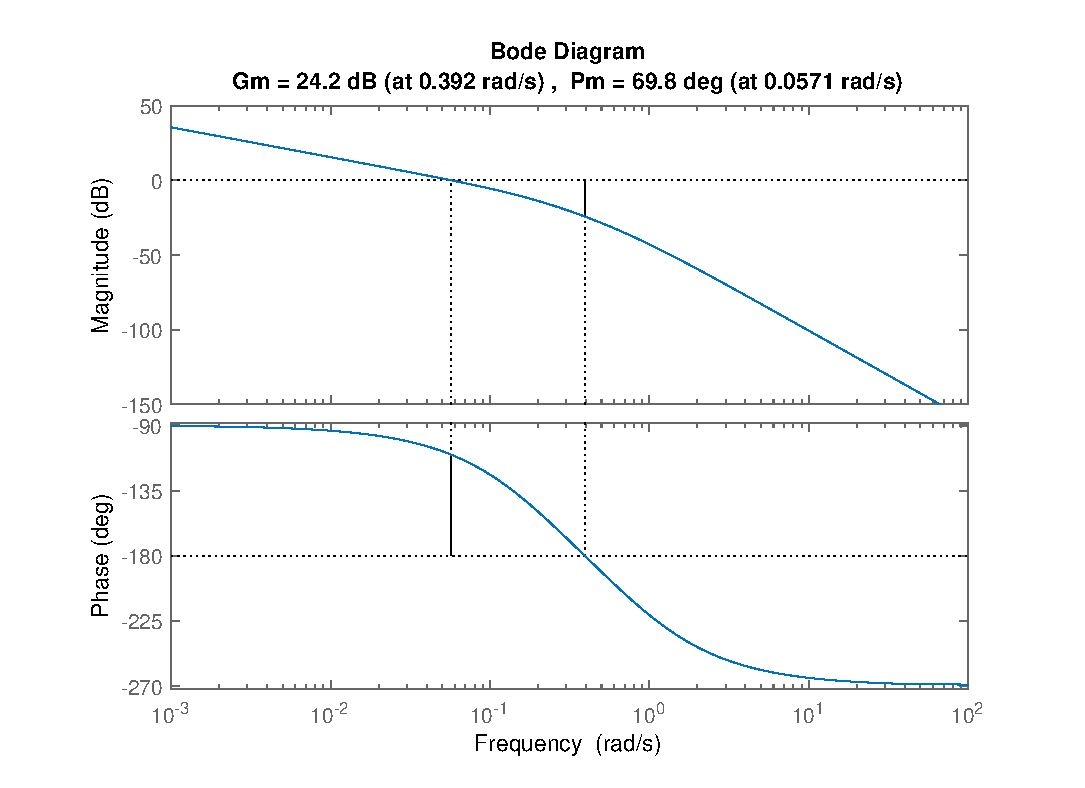
\includegraphics[scale=.70]{WOPI}
\caption(A PI szabályozóra tervezett nyitott kör Bode diagramja)
\end{figure}
A fázistartalék $\varphi_t=69.8^\circ$, ahol elértük a tervezett fázistartalékot.
Ezek utána zárt kör ugrásválasza:
\begin{figure}[H]
\centering
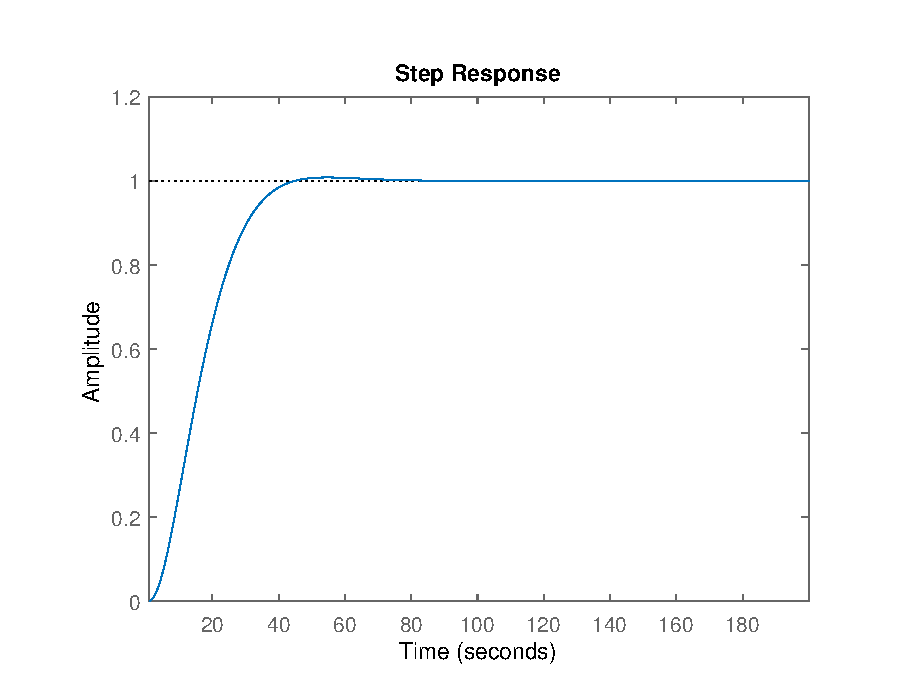
\includegraphics[scale=.70]{WCPI}
\caption(A PI szabályozóra tervezett zárt kör ugrásválasza)
\end{figure}
A rendszer stabil, nincs túllövése és nincs hiba és 1-re beáll.
\subsection{Közelítő PID szabályozó tervezés előírt fázistartalékra $\varphi_t=70^\circ$ és nulla állandósult hibára}
Első körben kiejtem a 2 leglassabb pólust ahol $\tau_1=12.4$ és $\tau_2=5$. Majd a $T_D$ Matlab alapján $T_D=3.30$. A $T_I$ pedig:
\[T_I=\tau_1+\tau_2-0.1T_D=17.069\]
Az előszabályozó $\frac{A_P}{T_I}=1$ esetén a nyitott köt átviteli függvény:
\[W(s)=\frac{2.33}{s^3+3.798s^2+2.33s}\]
Ebből a nyitott rendszerből megkerestem a vágási frekvenciát, ahol az $A_P=3.87$. Ezután a  $T_C=0.1*T_D=0.33$. A kiértékelések után a végleges átviteli függvényt létrehoztam a nyitott körre:
\[W(s)=\frac{0.5282}{s^3+3.798s^2+2.33s}\]
A ugrásválasz és a Bode diagramm:
\begin{figure}[H]
\centering
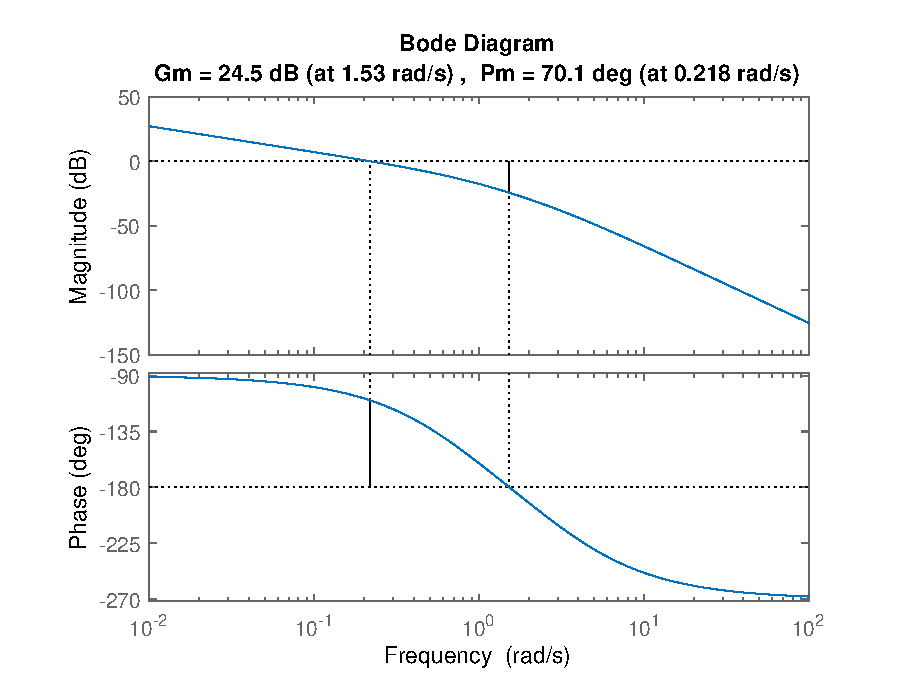
\includegraphics[scale=.70]{WOPID}
\caption(A PID szabályozóra tervezett nyitott kör bode diagramja)
\end{figure}
Lehet látni, hogy sikeresen elértük a fázistartalékot és 0.218 a vágási frekvencia.
\begin{figure}[H]
\centering
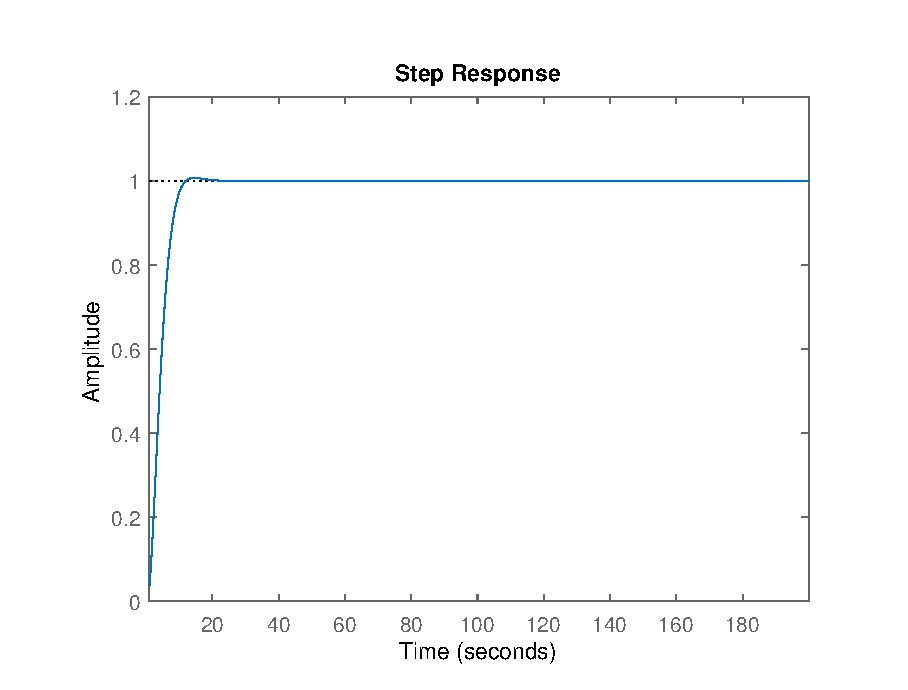
\includegraphics[scale=.70]{WCCP_PID}
\caption(A PID szabályozóra tervezett zárt kör ugrásválasza)
\end{figure}
Lehet látni, hogy rendszer stabil, egy nagyon minimális túllövése van és utána gyorsan beáll 1-re, ahol nem látok semmi hibajelet.
\subsection{Rendszerek összehasonlítása}
A tervezek rendszerek bode diagramja:
\begin{figure}[H]
\centering
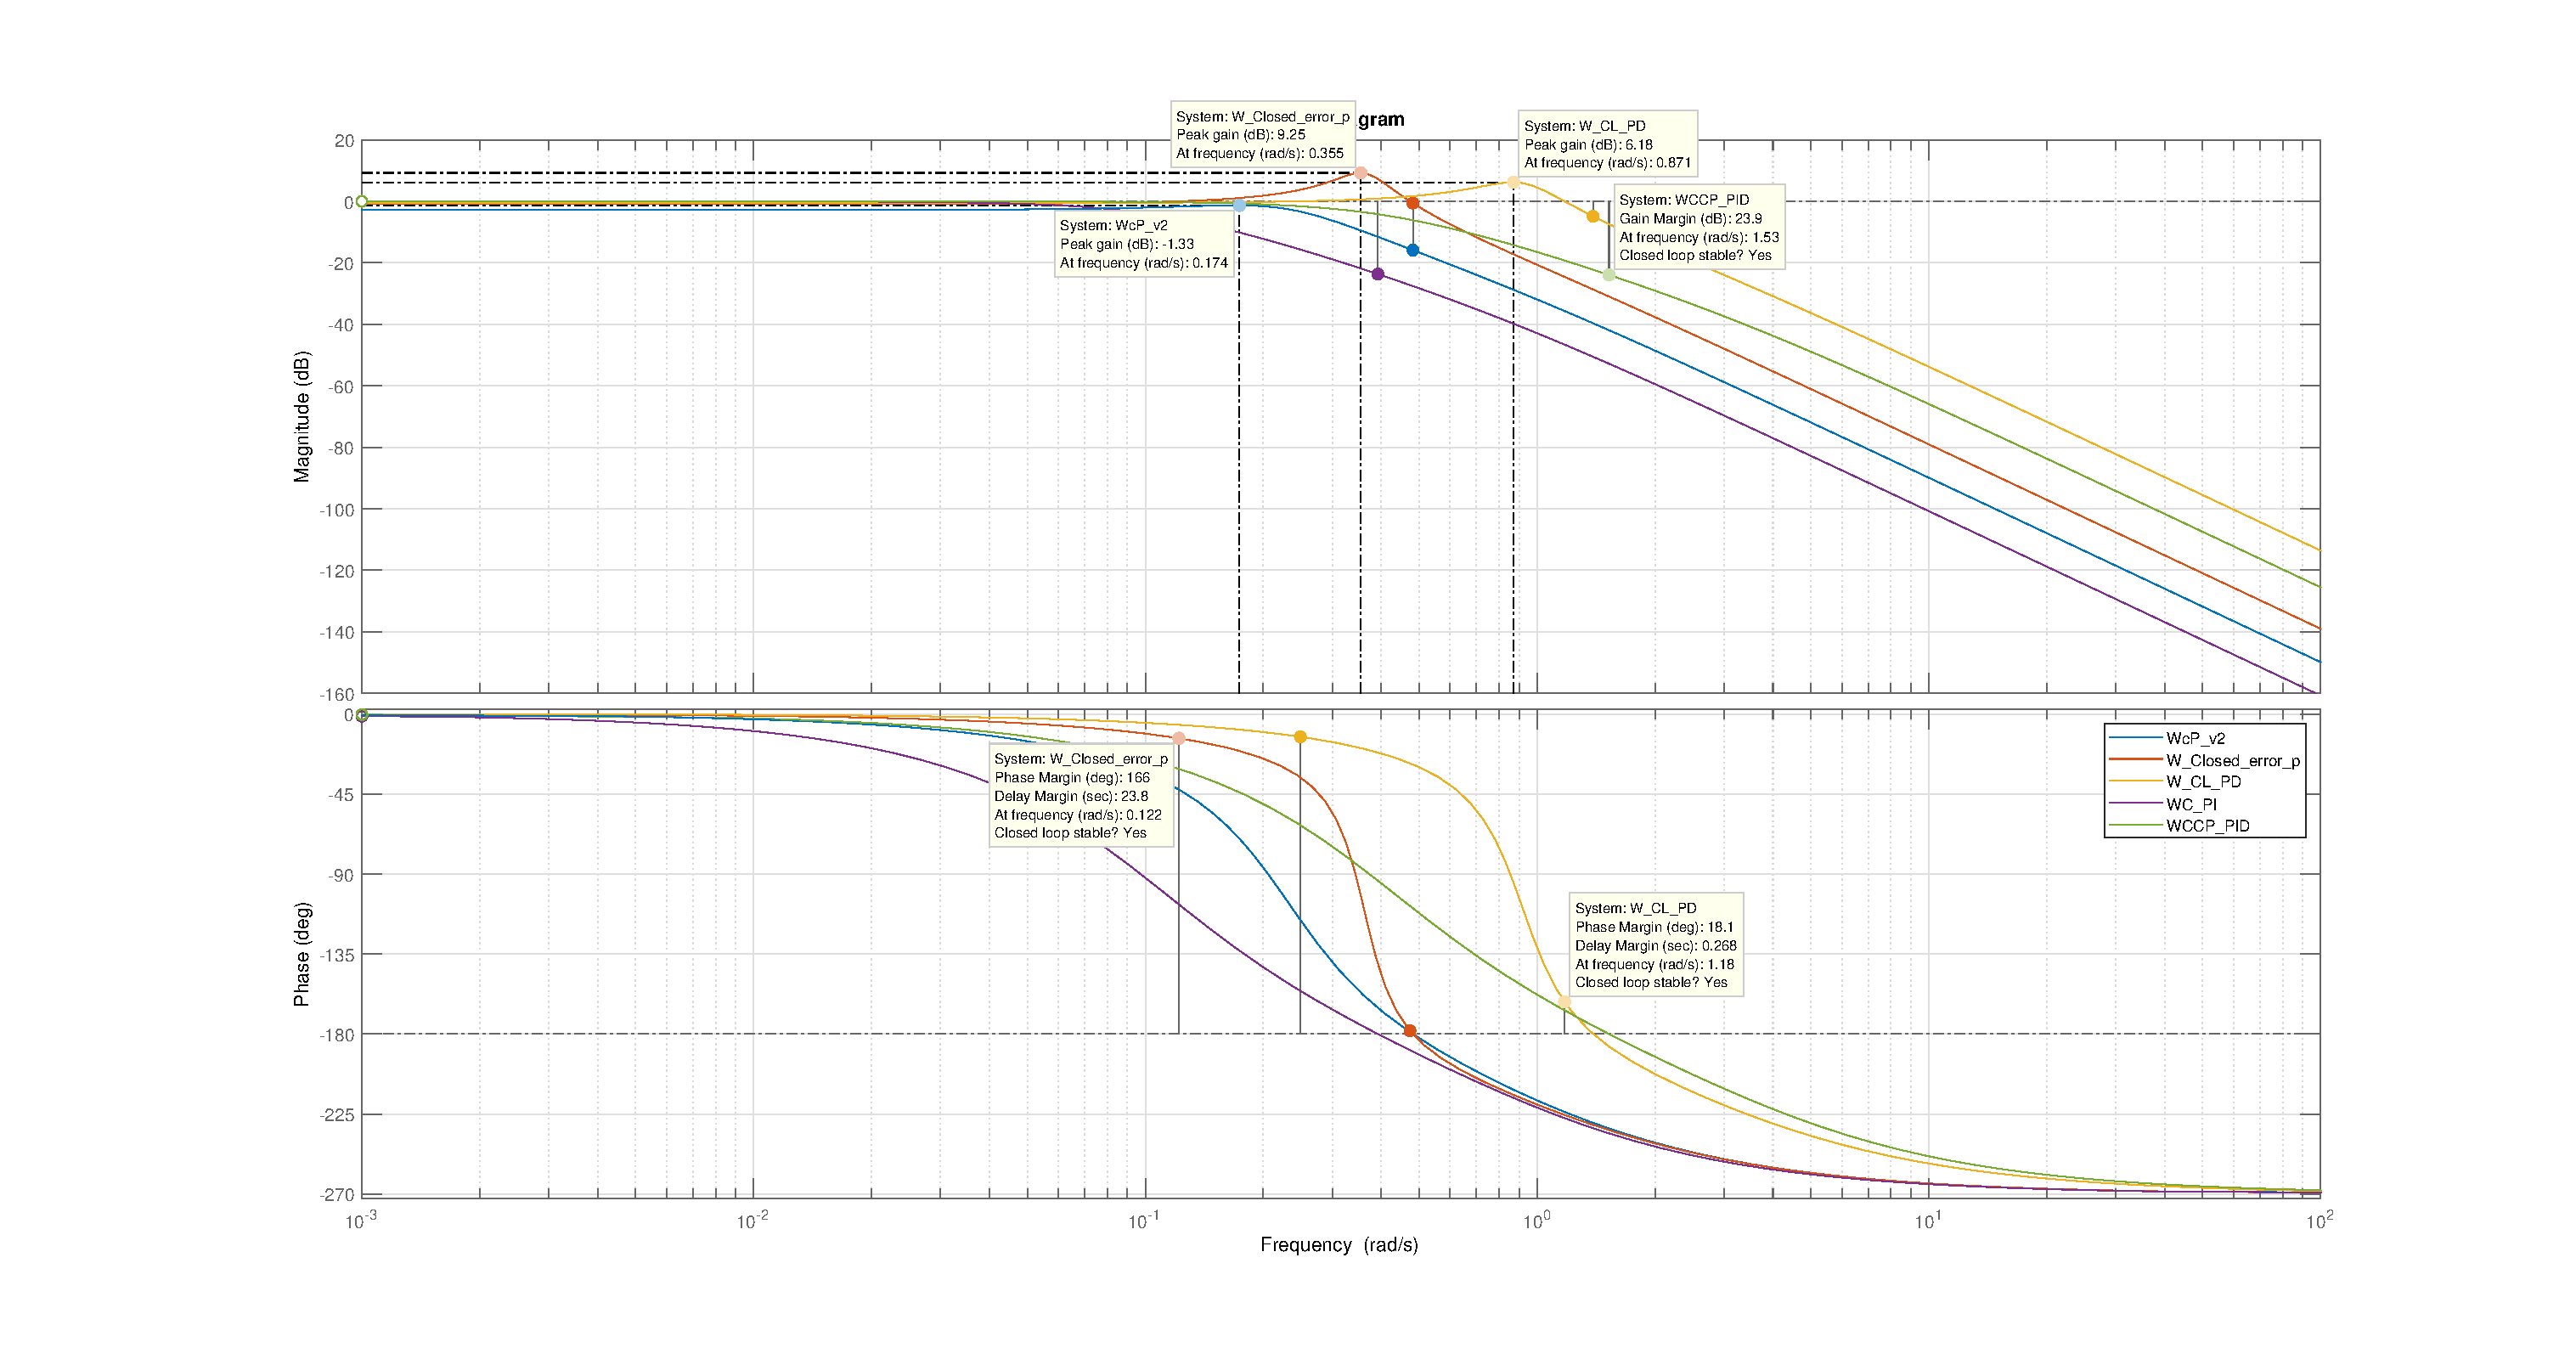
\includegraphics[width=180mm,height=140mm]{BODE_ALL}
\caption(A rendszerek bode diagramja)
\end{figure}
A rendszerek ugrásválasza:
 \begin{figure}[H]
\centering
\includegraphics[width=180mm,height=140mm]{STEP_ALL}
\caption(A rendszerek bode diagramja)
\end{figure}
Az ugrásválaszok alapján látható, hogy leggyorsabb rendszer a PD szabályozó lenne, viszont a túllövése több is van és magas is. A legjobb rendszer ami viszonylag gyors és stabil is az a közelítő PID szabályozó, ami miatt ez lenne a legjobb választás.
\end{document}